\chapter{Empirical evaluation}
\label{ch:evaluation}

% copied
    % The present parser is evaluated by comparing the text analysis it outputs with manually analysed text. The evaluation seeks to measure the parser \textit{precision} - i.e. how many segments have been produced by the parser that are also found in manual analysis; and the parser \textit{recall} - i.e. how many correct segments have been produced by the parser relative to the total number of produced segments.

    In order to count correct and incorrect number of segments they need to be matched first. This task is not trivial because there are errors in the corpus annotations (introduced below), a few differences in used grammars and a few divergences in treating certain linguistic phenomena - all of which are detailed below. For these reasons, slight deviations are tolerated in the annotation segment position provided that the label is the same and there is no other segment that constitutes a better match. The next two sections define segments and provide details on how and why they diverge. Section \ref{sec:segment-labels} describes how the segment labels differ and how they are mapped to extend the scope of the evaluation. 

    Identifying matches and near-matches between manual and automatic segments is well known in computer science as the Stable Marriage problem explained in Section \ref{sec:stable-marriage}. For the purpose of this evaluation I have implemented a variation of the Gale-Shapley algorithm \citep{Gale1962}. %Then, the section that follows, are finally described the empirical findings of the current evaluation. 

    % copied
    
    % In the current evaluation I use two sets of annotated texts. Table \ref{tab:corpus-sumary} summarises the corpora used for evaluation in this work. The first dataset (OCD) was created by Ela Oren and myself and is focused on syntactic constituency structure and clause MOOD features. The texts represent blog articles of people diagnosed with Obsessive Compulsive Disorder (OCD) who self-report on the challenge of overcoming OCD. 
    % %The dataset contains four texts comprising all together 988 clauses and 8605 words. 
    % The second dataset (OE1) is the result of PhD work of Anke Schultz \citep{schulz2015me} covering the Cardiff Transitivity analysis. It comprises 31 files spanning over 1503 clauses and 20864 words. In addition, she provided another similar smaller corpus (BTC) of 157 clauses that is also included into this evaluation. 

    % copied
    % \begin{table}[!ht]
    %     \centering
    %     \resizebox{\textwidth}{!}{%
    %     \begin{tabular}{|c|c|c|c|c|c|}
    %         \hline
    %         \textbf{Corpus} & \textbf{Elements} & \textbf{System Network} & \textbf{\begin{tabular}[c]{@{}c@{}}\# characters\\ (thousands)\end{tabular}} & \textbf{\# clauses} & \textbf{Annotator(s)}         \\ \hline
    %         OCD            & Syntax            & MOOD              & 16.2                                                                         & 147                 &  Ela Oren \& Eugeniu Costetchi \\ \hline
    %         OE1             & Semantics         & TRANSITIVITY      & 51.8                                                                         & 1503                & Anke Schultz                  \\ \hline
    %         BTC             & Semantics         & TRANSITIVITY      & 5.6                                                                          & 157                 & Anke Schultz                  \\ \hline
    %     \end{tabular}
    %     }
    %     \caption{Evaluation corpus summary}
    %     \label{tab:corpus-sumary}
    % \end{table}

    % The OE1 and BTC datasets were not developed for the purpose of evaluating constituency in the current parser but are compatible and can be adapted to evaluate the boundaries of constituent segments. They are primitively used for evaluation of the constituent's semantic function and some TRANSITIVITY features (to the degree provided in the corpus). To enable each of these evaluations the annotation data and parser output needed to be uniformly represented in order to be in alignment with the parser output. To achieve this, feature names were harmonised with the ones from PTDB following the same adjustments as described in Section \ref{sec:claning-ptdb}. In Section \ref{sec:results},  the empirical findings of the current evaluation are described.

\section{Segment definition}
% copied

%     To compare the segment boundaries we need to understand how they are represented in each output and how they can be brought to a common form comparison. 

%     \begin{minipage}{0.90\linewidth}
% \begin{lstlisting}[language=XML,frame=single,caption=Segment example in UAM corpus tool,label=lst:segment1]
% <segment id="4" start="20" end="27" 
% features="configuration; relational; attributive" 
% state="active"/>
% \end{lstlisting}
%     \end{minipage}
%     All datasets were created with the UAM Corpus Tool \citep{ODonnell2008,ODonnell2008a} version 2.4. The annotations, in this software, are recorded as segments spanning from a start to an end position in the text file together with the set of features (selected from a systemic network) attributed to that segment. There are no constituency or dependency relations between segments. The XML representation of an example annotation segment is provided in Listing \ref{lst:segment1}. There the \textit{id} attribute indicates the unique identification number within the annotation dataset, the \textit{start} and \textit{end} attributes define the segment between two character offsets relative to the beginning of the text file. 
    
% copied

% \begin{minipage}{0.90\linewidth}
% \begin{lstlisting}[numbers=left, stepnumber=1,firstnumber=0,frame=single,caption=Raw text example in annotation data,label=lst:exampleText,escapeinside={(*}{*)}]
% (*\textcolor{black!50}{$_{0}$}*)Red riding hood excerpt(*\textcolor{black!50}{$_{24}$}*)
% (*\textcolor{black!50}{$_{25}$}*)"What have you in that basket,   Little Red Riding Hood?"(*\textcolor{black!50}{$_{82}$}*)
% (*\textcolor{black!50}{$_{83}$}*)
% (*\textcolor{black!50}{$_{84}$}*)"Eggs and butter and cake, Mr. Wolf."(*\textcolor{black!50}{$_{111}$}*)
% \end{lstlisting}
% \end{minipage}

% Listing \ref{lst:exampleText} presents an example raw text from the annotation dataset containing an initial title line and two sentences separated by an empty line. The greyed index numbers at the beginning and end of each line indicate character offsets. In some files, the first line plays the role of a header containing the title or the file name. In this example it is a title. Either way, this first line is neither considered for annotation nor parsing. Some files contain one sentence per line, others separate sentences by an extra blank line and in some the text is one continuous block. The text may  contain sporadically tabs and blank spaces such as here in line 1 between the comma and the ``Little Red Riding Hood''. 

    Parsimonious Vole parses sentences one by one and not the whole text at once. Before parsing, the document is chunked into sentences guided by the punctuation delimiters. In addition, the Stanford dependency parser normalises the input text by trimming spaces and tabs, adjusting character encoding and replaces some special characters such as quotes, brackets, punctuation, etc.

    Listing \ref{lst:exampleTextPreprocessed} presents the preprocessed text before it is parsed. The title line is cropped from the file. Each line contains a separate sentence. The text is tokenised such that words and punctuation marks are separated by a single space.

\begin{lstlisting}[numbers=left, stepnumber=1,firstnumber=0,frame=single,caption=Parser preprocessed text example ,label=lst:exampleTextPreprocessed,escapeinside={(*}{*)}]
(*\textcolor{black!50}{$_{0}$}*)" What have you in that basket , Little Red Riding Hood ? "(*\textcolor{black!50}{$_{60}$}*)
(*\textcolor{black!50}{$_{61}$}*)" Eggs and butter and cake , Mr. Wolf . "(*\textcolor{black!50}{$_{102}$}*)
\end{lstlisting}

    \begin{figure}[!ht]
        \centering
        \begin{tikzpicture}[pattern-node]
        \node[pattern-node] (s0) {25};
        \node[pattern-node, right = 11em of s0] (e0) {82};
        \draw[edge-style] (s0) -- (e0) node[midway, above]{57};
        \node[pattern-node, right = 0.1em of e0] (s1) {83};
        \node[pattern-node, right = 7em of s1] (e1) {120};
        \draw[edge-style] (s1) -- (e1) node[midway, above]{37};
        
        \node[pattern-node, xshift=-2.5em, below = 1em of s0] (ss0) {0};
        \node[pattern-node, right = 12em of ss0] (se0) {60};
        \draw[edge-style] (ss0) -- (se0) node[midway, above]{60};
        \node[pattern-node, right = 0.1em of se0] (ss1) {61};
        \node[pattern-node, right = 8em of ss1] (se1) {102};
        \draw[edge-style] (ss1) -- (se1) node[midway, above]{41};
        \end{tikzpicture}
        \caption{Graphic representation of sentence segment misalignment between Listing \ref{lst:exampleText} and Listing \ref{lst:exampleTextPreprocessed} }
        \label{fig:segment-misalignment}
    \end{figure}

    After the parser preprocessing process, the input and output texts are no longer identical. The sentence and word offsets are no longer reliably defined with respect to the original text and therefore the segments need to be matched. There are two fundamental kinds of segment misalignments: the segment offset shifting and segment resizing (either shrinking or enlarging). Sometimes it can also be a combination of the two. The Allen interval algebra \citep{Allen1983} systematises thirteen basic relations to position segments relative to each other. Nonetheless, in the current work we are not interested in investigating segment offset shifts but rather what would be an efficient way to match them independently of their position or misalignment.

    To make manual and automatic annotations comparable, the constituency graphs need to be reduced to a set of segments corresponding to each constituent. The first task of the evaluation is to find matches or near-matches between two segment bundles; this is addressed in the next section.

\section{From rich constituency graphs to evaluation segments}
\label{sec:segment-alignment}
    % copied
    
    % In this section I describe the task of generating from rich constituency graphs (CG) segments that are similar if not identical to those in the corpus. If we ignore the set of associated labels (systemic features), which we will consider in the next section, then two segments are considered identical when (a) their start and end indexes and (b) the text in between are identical.

    % To fulfil this task, the text processed by the parser is re-indexed back into the original raw text at the level of words (tokens), constituents and sentences. Algorithm \ref{alg:re-index-text} provides pseudo-code of the indexing process.

    % \begin{algorithm}[!ht]
    %     \Input {CG bundle, \text} %, \dg
    %     \Begin {
    %         offset $\leftarrow$ 0\;
    %         \For{\cg \KwTo CG bundle}
    %         {
    %             generate segments for \cg indexed on \text given the offset\;
    %             offset $\leftarrow$ the end of \cg\;
    %         }
    %     }
    %     \caption{Algorithm to generate segments for the CG bundle indexed on the raw text}
    %     \label{alg:re-index-text}
    % \end{algorithm}

    % The input for Algorithm \ref{alg:re-index-text} is a set of constituency graphs produced by the parser and the original text. The result of this algorithm is a set of segments indexed according to the raw text by iterating the resulting constituency graphs one by one and indexing each with respect to the offset given by the previous one. 

    % \begin{algorithm}[!ht]
    %     \Input {\cg, \text, sentence offset} %, \dg
    %     \Begin {
    %         words $\leftarrow$ get \cg the list of words \;
    %         \For{\word \KwTo list of sentence word segments}
    %         {
    %             find the \word in the \text after a given sentence offset\;
    %             \eIf{\word found}
    %             {
    %                 start $\leftarrow$ get first word start index\;
    %                 end $\leftarrow$ get the last word end index\;
    %                 create a new segment (start, end, \word)\;                
    %             }
    %             {
    %                 generate a warning (manual adjustment needed)\;
    %             }
    %         }
    %         \For{\node \KwTo \cg in BFS postorder}
    %         {
    %             find the word span of the constituent\;
    %             start $\leftarrow$ get first word start index\;
    %             end $\leftarrow$ get the last word end index\;
    %             labels $\leftarrow$ get \node class, function and features\;
    %             create new segment (start, end, labels)\;
    %         }
    %         \Return set of segments\;
    %     }
    %     \caption{Algorithm to generate segments for CG constituents indexed on the raw text}
    %     \label{alg:re-index-words-and-cg}
    % \end{algorithm}

    % The way each CG is indexed is described by Algorithm \ref{alg:re-index-words-and-cg}, which returns a set of segments from the constituency graph considering a given offset. First a token level indexing is performed and corresponding segments generated. Then for each CG constituent, segments are generated based on its word span. The indexes are set from beginning of the first word to the end of the last word. The labels of the segment are the CG class, functions and systemic features discussed in the next section.

    % \begin{equation} \label{eq:distance}
    % d= \sqrt{(start_S - start_T)^{2}+(end_S-end_T)^{2}}
    % \end{equation}
    
    % \begin{equation} \label{eq:distance-simpliefied}
    % d= \sqrt{\varDelta_{start} ^{2}+\varDelta_{end}^{2}}
    % \end{equation}

    % copied

    Later in this chapter I address how the manually created segments and parser generated segments are aligned. 
    % Here it is noteworthy to mention that the manually created segments contain errors. Some segments are either shifted and include the adjacent spaces or, the converse, leave out one or two characters of a marginal word. 
    For this reason the segment alignment process needs to tolerate a certain distance between the stand/end indexes of aligned segments. I adopted the geometric distance to measure the difference between the segment start and end indexes. For two segments $S(start_S,end_S)$ and $T(start_T,end_T)$ the geometric distance is defined in Equation \ref{eq:distance}. We can replace the difference between start and end indexes with $\varDelta_{start}$ and $\varDelta_{end}$ notation and obtain the reduced form provided in Equation \ref{eq:distance-simpliefied}.

\section{Considering the segment labels}
\label{sec:segment-labels}

    
    Provided that the task of indexing the segment indexes and content such that they ``roughly'' correspond to each other has been done we need to compare the segment labels. However the labels of manually created segments differ from the segments provided by the parser. Besides the shift in the offset mentioned above, another difference is in number of ascribed segments. In many instances, the manual annotation is less delicate and thus contains fewer features than the one provided by the parser. Still, some of the manual annotations contain features that are not provided by the parser (i.e. not yet implemented), such as the Thematic structure of the clause or the Modal Assessment features. 

    % To address this issue, in the current evaluation, the segments are reduced to carry only one label. The consequence is that segments with multiple features (Figure \ref{fig:segment-multiple}) are broken down into multiple segments with the same span (Figure \ref{fig:segment-simple}) for each feature. When each segment contains exactly one feature the evaluation can be focused on one or a set of features of interest by selecting only the segments that contain exactly those. 

    % \begin{figure}[!ht]
    %     \centering
    %     \begin{subfigure}[b]{0.47\textwidth}
    %         \centering
    %         \begin{tikzpicture}[pattern-node]
    %         \node[pattern-node] (start) {20};
    %         \node[pattern-node, right = 7em of start] (end) {27};
    %         \draw[edge-style] (start) -- (end) node[midway, above]{configuration,\\relational,\\attributive};
    %         \end{tikzpicture}
    %         \caption{A segment with a set of features}
    %         \label{fig:segment-multiple}
    %     \end{subfigure}
    %     \begin{subfigure}[b]{0.47\textwidth}
    %         \centering
    %         \begin{tikzpicture}[pattern-node] 
    %         \node[pattern-node] (start1) {20};
    %         \node[pattern-node, right = 7em of start1] (end1) {27};
    %         \draw[edge-style] (start1) -- (end1) node[midway, above]{configuration};
            
    %         \node[pattern-node, below = 1em of start1] (start2) {20};
    %         \node[pattern-node, right = 7em of start2] (end2) {27};
    %         \draw[edge-style] (start2) -- (end2) node[midway, above]{relational};
            
    %         \node[pattern-node, below = 1em of start2] (start3) {20};
    %         \node[pattern-node, right = 7em of start3] (end3) {27};
    %         \draw[edge-style] (start3) -- (end3) node[midway, above]{attributive};	
    %         \end{tikzpicture}
    %         \caption{A set of segments with single features}
    %         \label{fig:segment-simple}
    %     \end{subfigure}
    %     \caption{Example of breaking down a segment with multiple features into set of segments with a single feature}
    %     \label{fig:segment-breackdown}
    % \end{figure}

    There are more differences in the grammar and annotation style between the manual and automatic processes. This means that both structure and feature names provided by the system networks differs. It was already mentioned above that the THEME system network is not implemented in the current version of the parser but is provided in some manual annotations. 

    %Also there are some differences in the constituency structure itself. For example in the treatment of conjunction (discussed in Section \ref{sec:coordination}) or the verb phrase. The next section presents the main differences in detail. 
    
    %\section{Considering the annotation methodology}
    %In this section I provide some key differences in how corpus has been annotated as compared to parser output.
    
    % copied
    
    % %The differences to parser
    % In the corpus, punctuation marks such as commas, semicolons, three dots and full stops are not included in the constituent segments while the parser includes them at the end of each adjacent segment. None of the conjunctions (such as ``and'', ``but'', ``so'', etc.) are included in the conjunct segments; they are considered markers in the clause/group complexes rather than part of the constituent. The treatment of conjunction is discussed in Section \ref{sec:coordination}. The parser, on the other hand, includes the conjunctions in the following adjacent segment. Moreover the conjuncts spans differ as well. Instead of being annotated in parallel, as depicted in Figure \ref{fig:segment-conjunction-paralel}, the segments are subsumed in a cascade from the former to the latter as depicted in Figure \ref{fig:segment-conjunction-subsumed}. 

    % \begin{figure}[!ht]
    %     \centering
    %     \begin{subfigure}[b]{0.47\textwidth}
    %         \centering
    %         \begin{tikzpicture}[pattern-node]
    %         \node[pattern-node] (start) {};
    %         \node[pattern-node, right = 5em of start] (end) {};
    %         \draw[edge-style] (start) -- (end) node[midway, above]{conjunct 1};
            
    %         \node[pattern-node, right = .5em of end] (conj) {and};
            
    %         \node[pattern-node, right = .5em of conj] (start1) {};
    %         \node[pattern-node, right = 5em of start1] (end1) {};
    %         \draw[edge-style] (start1) -- (end1) node[midway, above]{conjunct 2};
            
    %         \end{tikzpicture}
    %         \caption{Conjuncts annotated as parallel segments}
    %         \label{fig:segment-conjunction-paralel}
    %     \end{subfigure}
    %     \quad
    %     \begin{subfigure}[b]{0.47\textwidth}
    %         \centering
    %         \begin{tikzpicture}[pattern-node] 
    %         \node[pattern-node] (start) {};
    %         \node[pattern-node, right =14em of start] (end) {};
    %         \draw[edge-style] (start) -- (end) node[midway, above]{conjunct 1};
            
            
    %         \node[pattern-node, below = 0.1em of end] (end1) {};
    %         \node[pattern-node, left = 8em of end1] (start1) {};
    %         \draw[edge-style] (start1) -- (end1) node[midway, above]{conjunct 2};
            
    %         \node[pattern-node, below = -0.6em of start1, xshift=1.8em] (conj) {and};        
            
            
    %         \end{tikzpicture}
    %         \caption{Conjuncts annotated as subsumed segments}
    %         \label{fig:segment-conjunction-subsumed}
    %     \end{subfigure}
    %     \caption{Treatment of conjunctions in the corpus compared to the parser}
    %     \label{fig:conjunction-treatment}
    % \end{figure}

    %no more apparently, neither identical to Cardiff grammar, but close.
    %Another difference is the way verbs and verb groups are handled. In the parser is implemented the Sydney Grammar's Finite and Predicate constituents while the corpus is annotated according to Cardiff Grammar with Main Verbs, Finite, Auxiliary, Negation Particles etc. as explained in Section \ref{sec:discussion-unit-classes}.

    The differences in the grammar are due to variations in the feature names and in the system network structure. For example the element names are spelled differently ``predeictic'' and ``pre-deictic'', ``root'' and ``clause'' or ``explative-marker'' and ``expletive''. Similar spelling variations are present in the feature names - for example ``two role'' and ``two-role-action'' and other variations alike. To remedy this issue the current evaluation establishes mappings between the manual and automatically generated features. 

    Now that the main divergences have already been outlined, I explain how the stable matches between the segments are established.

\section{Aligning corpus to parse segments}
\label{sec:stable-marriage}
    % %When we take the segment label into consideration then, 
    
    % copied
    
    % The task of aligning two sets of labelled segments is almost the same as the well know problem in computer science called \textit{stable marriage problem} \citep{Gusfield1989}. The standard enunciation of the problem is provided below and is solved in an efficient algorithm named Gale-Shapley \citep{Gale1962} after its authors.

    % copied

    % \begin{quotation}
    %     Given \textit{n} men and \textit{n} women, where each person has ranked all members of the opposite sex in order of preference, marry the men and women together such that there are no two people of opposite sex who would both rather have each other than their current partners. When there are no such pairs of people, the set of marriages is deemed stable \citet{iwama2008}.
    % %    \footnote{see \href{https://en.wikipedia.org/wiki/Stable_marriage_problem}{stable marriage problem on Wikipedia}}
    % \end{quotation}

    %%There is however a difference between the stable marriage and the current segment matching problem. The standard stable marriage problem assumes that the preferences of each individual woman and men for the opposite sex are known and expressed as a complete ordered list.

    % copied
    % In the context of this evaluation the group of men is associated with the segments generated automatically by the parser and the group of women with the segments available from the manual analysis. 

    % The standard stable marriage problem is formulated such that there is a group of men and a group of women and each individual from each group expresses their preferences for every individual from the opposite group as an ordered list. The assumption is that the preferences of every individual are known and expressed as a complete ordered list of individuals from the opposite group ranging from the most to the least preferred one. Thus the preference list must be \textit{complete} and \textit{fully ordered}. 

    % To fulfil these requirements I construct a distance matrix from each automatically created segment to every manually created one. The distance measure considered here is the Euclidean one provided in Equation \ref{eq:distance-simpliefied} above. The matrix represents the complete and fully ordered set of preferences stipulated in the original problem formulation. In addition to having identical offsets, the segments need to carry the same labels in order to be considered a match. This condition is not expressed in the original problem but is considered in Algorithm \ref{alg:matching}.

    %%which none of these constraints can be fulfilled in the context of the present evaluation. 
    %%According to \citet{iwama2008} this version of the problem is called \textit{Stable Marriage with Ties and Incomplete List} (SMTI) addressed first by \citet{irving1994stable}. 
    %%To fulfil these requirements I construct the preferences matrix between every segments of the second group
    %%Next I explain the identity criteria between two segments which further clarifies the problem to be solved.

    % copied
    % \begin{algorithm}[!ht]
    %     \Input{\aslist, \mslist} %, \dg
    %     \Begin{
    %         mark all \aslist and \mslist free\;
    %         compute distances from each \mslist to every \aslist\;
    %         \While{$\exists$ free \aslist}{
    %             \as $\leftarrow$ first free from \aslist\;
    %           \If{$\exists$ \mslist not yet tested to match \as}{
    %               \ms $\leftarrow$ the nearest among \mslist to \as with identical label \;
    %               \If{\ms is free}{
    %                   match \as and \ms \;
    %                   mark \as and \ms as non-free \;
    %               }               
    %           \Else{
    %                   $\as'$ $\leftarrow$ the current match of \ms \;
    %                   \If{\as is closer to \ms than $\as'$}{
    %                       match \as and \ms \;
    %                       mark \as and \ms as non-free \;
    %                       mark $\as'$ as free \; 
    %                   }
    %               }
    %           }
    %           \Else{
    %               mark \as as non-free and non-matching \;
    %           }
    %         }
    %     }
    %     \caption{The algorithm for matching automatic and manual segments}
    %     \label{alg:matching}
    % \end{algorithm}

    The input to the algorithm is the set of automatically generated segment list \aslist and the manually created segment list \mslist.  It begins with initialising all the segments as \textit{free} meaning that none of them are matched yet (originally married). The segments can be marked either as \textit{non-free matching} or \textit{non-free non-matching}. A part of the initialisation is also the creation of the distance matrix mentioned above representing a complete and ordered set of preferences for each segment. 

    The algorithm iterates over the \aslist for as long as there exist free ones. If there exists a \ms (manually created segment) which has not been attempted to match \as; then the algorithm attempts matching \as to the nearest \ms that has the same label. If \ms is free then it is a match. Otherwise compare \as to $\as'$ (currently assigned match of \ms) and then consider a match with the nearest one (i.e. shortest distance). When there are no \mslist to test mark \as as non-free and non-matching meaning that it shall no longer be considered by the algorithm.

    In the end the algorithm provides a list of successful matches out of which we can also deduce which \aslist and \mslist have not been matched. The next section provides the empirical measurements resulting from applying this method. 

\section{Evaluation statistics}
\label{sec:results}

    In this section I present a series of measurements addressing two quality criteria of the parser. Firstly, the degree of divergence in segment spans between manual and parsed segments in all corpora (OCD, BTC and OE1). And secondly, the accuracy of the parser with respect to manual annotations measured through precision, recall and F_1 measures. The syntactic constituency and some MOOD features are derived from the OCD corpus only, followed by the semantic constituency and TRANSITIVITY features evaluation based on OE1 and BTC corpora. 

\subsection{Segment divergence: general findings}

    The segments don't perfectly align, as described in previous sections, due to minor differences in annotation approach, text normalisation and trimming before parsing (that was not performed before the manual annotation), errors in the annotations (missing or including characters). The misalignment is measured using the geometric distance 
    %$d= \sqrt{\varDelta start ^{2}+\varDelta end ^{2}} $ 
    on segments matched by Algorithm \ref{alg:matching}. The presented statistics are calculated on a number of over 12500 segment pairs whose mean distance is 4.84 with a standard deviation of 14.51. The distance is distributed between a minimum 0 and maximum 219 characters. The mean values is close to the minimum point and standard deviation is fairly large which indicates that most of the data points are situated between 0 and slightly over the mean continued by a very long tail of rare and distant data points. This intuition can be seen in the histogram depicted in Figure \ref{fig:segment-distance-histogram-full} below. This dataset resembles the Pareto distribution where 74\% are not shifted at all or 83\% of the segments are slightly shifted up to 5 characters.

\begin{figure}[!ht]
    \centering
    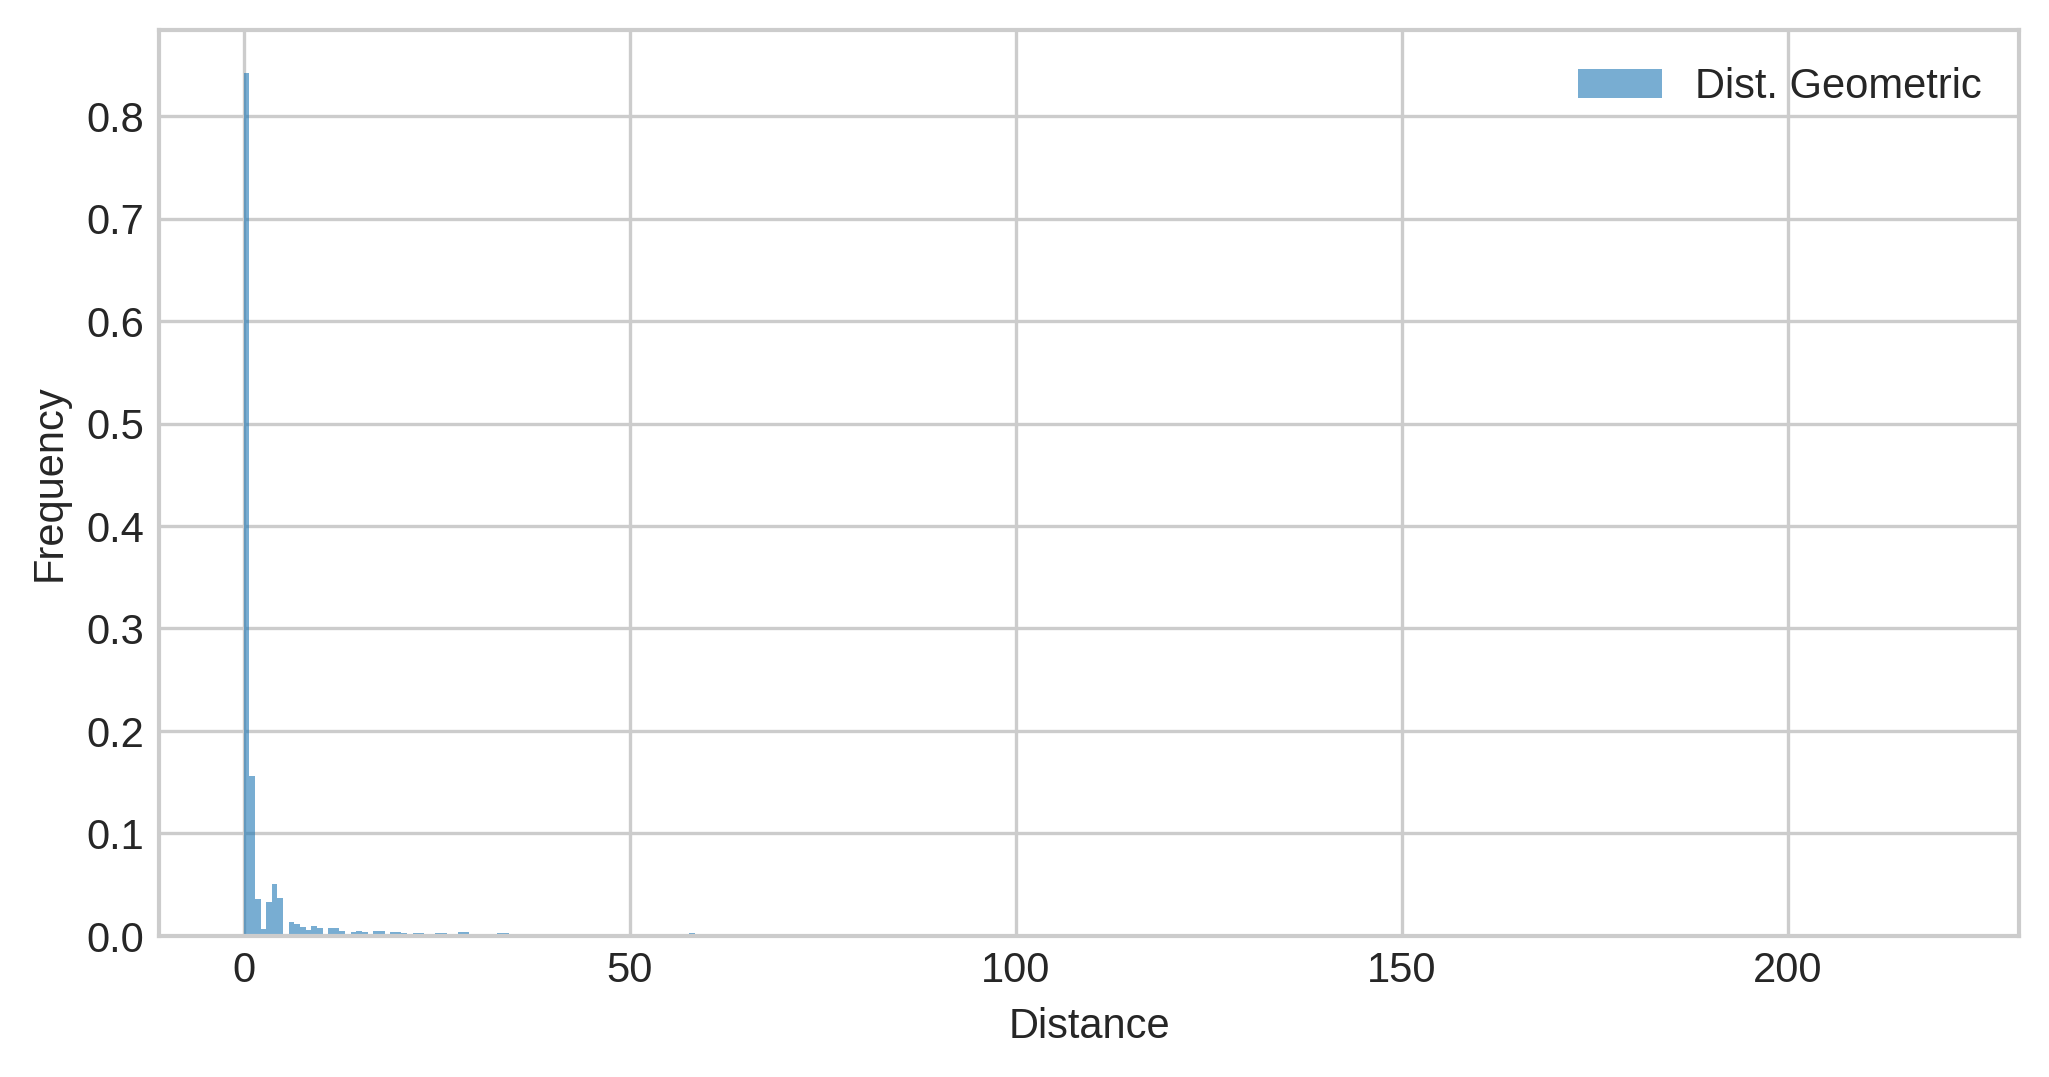
\includegraphics[width=.65\textwidth]{evaluation-results/figures/distance-distr-histogram-full}
    \caption{Full histogram of the distance distribution of the matched segments (binning=300)}
    \label{fig:segment-distance-histogram-full}
\end{figure}

    Because of a very long tail, I reduce the further analysis to the distance span between 0 and 40. Figure \ref{fig:segment-distance-distribution} depicts the histogram of distances between matched segments (in 300 bins). It shows that most segments (89\%) are cumulated in first two bins with distance up to 2. The consequent three bins also contain a significant portion of segments with distance up to 5. The rest of the bins, representing a very long tail, span distances up to maximum 219 and containing a small amount of segments. 

    \begin{figure}[!ht]
        \centering
        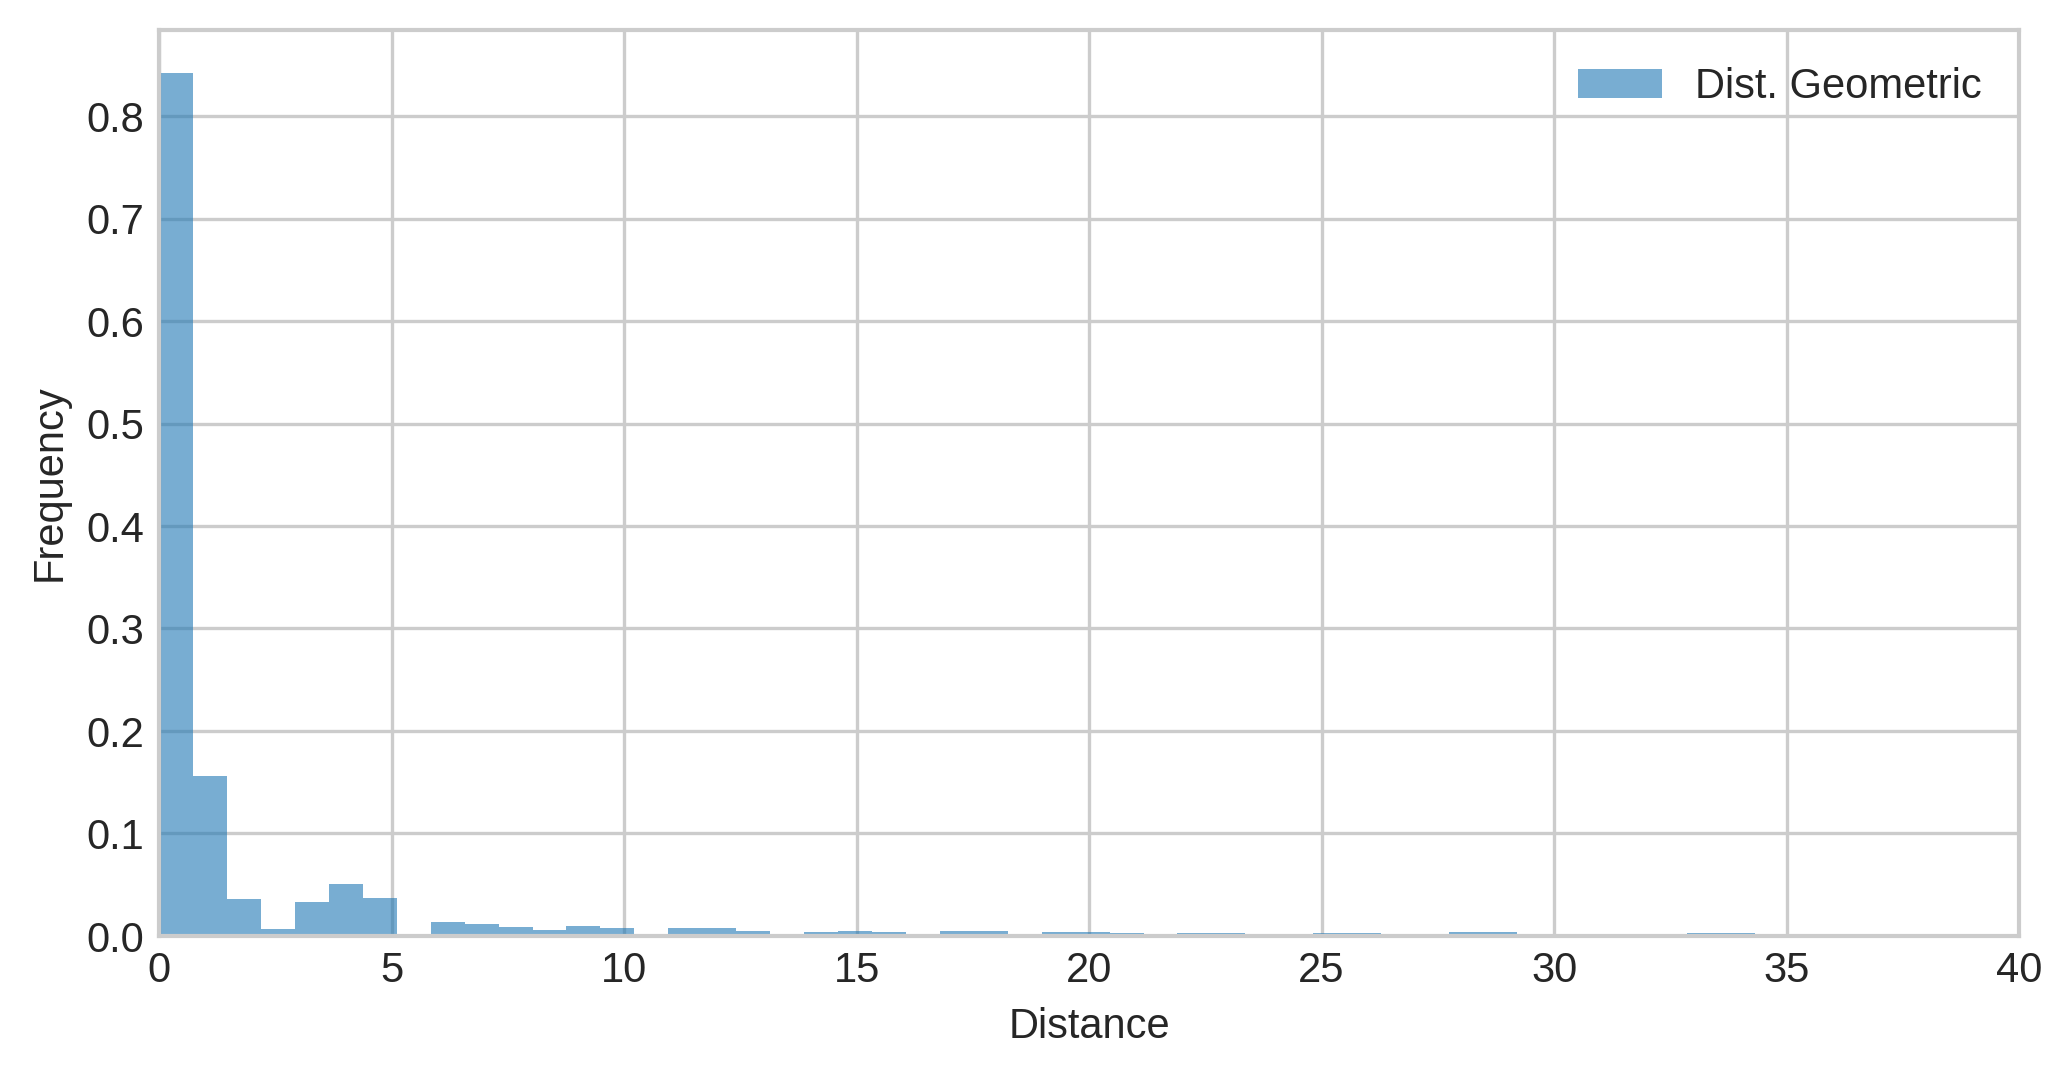
\includegraphics[width=.65\textwidth]{evaluation-results/figures/distance-distr-histogram}
        \caption{Reduced histogram of the distance distribution of the matched segments (binning=300). View reduced to the a distance of 40 characters}
        \label{fig:segment-distance-histogram}
    \end{figure}

    This distribution can be viewed in its cumulative form depicted in Figure \ref{fig:segment-distance-distribution}. Here we see that over 51\% of segments are perfectly aligned. 80\% of the segments are slightly shifted up to a distance of maximum 5 characters. This can be explained by differences in (a) punctuation, (b) conjunction and (c)verbal group treatment described above. The next 5\% of the segments are shifted between 5 and 10 characters. The last 10\% cover the heavy shift of distances 20 to 219. This may be due to differences in verbal group treatment, subsumed conjuncts (clause and group conjunctions) and erroneous prepositional phrase attachment (treated as Qualifier instead of Complement/Adjunct or vice versa). 

    \begin{figure}[!ht]
        \centering
        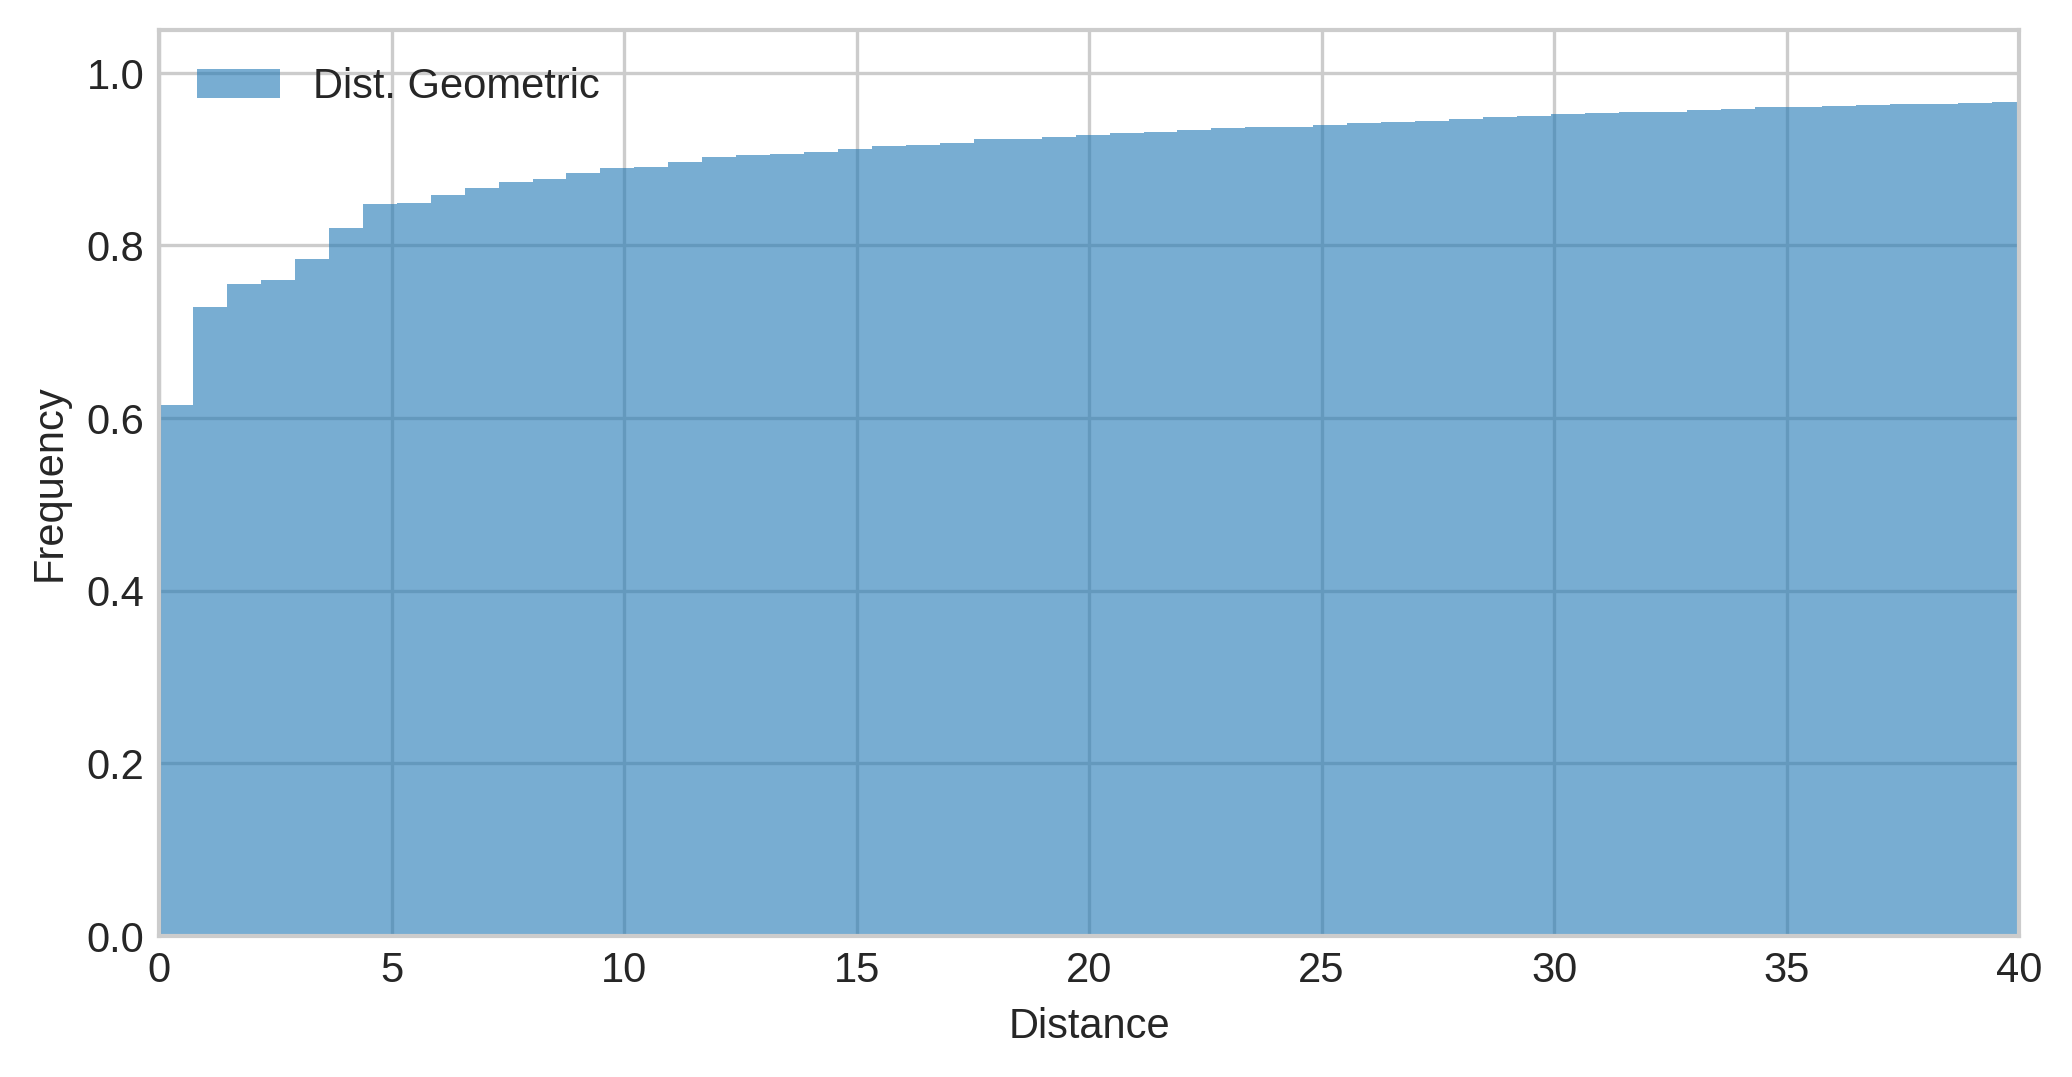
\includegraphics[width=.65\textwidth]{evaluation-results/figures/distance-distr-cumulative}
        \caption{Cumulative histogram of the distance distribution of the matched segments (binning=300). View reduced to the a distance of 40 characters}
        \label{fig:segment-distance-distribution}
    \end{figure}

\subsection{Segment divergence breakdown by element type}

    If we take a closer look at Figure \ref{fig:segment-distance-histogram} we notice some spikes and a tendency towards some local values. What would the histogram look like if we group values in a different manner considering these spikes and the long tail of the distribution. In Figure \ref{fig:segment-distance-histogram} we can observe several dips at around distances 3, 6, 11, 13, 17, 19, 22, 24 and so on. I decided to consider these dips for deciding bin borders in the new bin design. And, since the tail is very long with very few values, as the bins advance to the left, each is designed over longer span this way compressing the tail. In Table \ref{tab:progressive-bins} is presented such binning design. Also each interval is assigned a category that means the degree of deviation.

    \begin{table}[!ht]
        \begin{tabular}{|c|c|c|c|c|c|c|}
            \hline
            \textbf{degree}          & insignificant & tiny & little & moderate & significant & high   \\ \hline
            \textbf{distance intervals} & 0-3           & 3-5  & 5-10   & 10-20    & 20-50       & 50-250 \\ \hline
        \end{tabular}
        \caption{The progressive binning scale considering the dataset properties}
        \label{tab:progressive-bins}
    \end{table}

    Besides custom binning described above, looking at each segment label in part brings more clarity to the evaluation. The most relevant segment labels are the unit elements. In the current evaluation, the annotators provide clause level syntactic (Subject, Complement, Adjunct, Main verb, Finite) and semantic (Configuration, Main verb, Participant role) elements. These elements are used so a dimension in the breakdown of the segment divergence that follows. 

    Using the bins defined in Table \ref{tab:progressive-bins} the distribution of segment deviations grouped by the main syntactic elements is provided in Table \ref{tab:deviation-per-feature-and-degree-constit} that is also depicted in Figure \ref{fig:segment-distance-degree-features-mood}. 

    
    \begin{table}[!ht]
        \resizebox{0.98\linewidth}{!}{%
        \begin{tabular}{|c|c|c|c|c|c|c|}
            \hline
            \multirow{2}{*}{\textbf{element}} & \multicolumn{6}{c|}{\textbf{\% of segments per degree of deviation}} \\ \cline{2-7} 
            & \textbf{\begin{tabular}[c]{@{}c@{}}insignificant\\ (0-3)\end{tabular}} & \textbf{\begin{tabular}[c]{@{}c@{}}tiny\\ (3-5)\end{tabular}} & \textbf{\begin{tabular}[c]{@{}c@{}}little\\ (5-10)\end{tabular}} & \textbf{\begin{tabular}[c]{@{}c@{}}moderate\\ (10-20)\end{tabular}} & \textbf{\begin{tabular}[c]{@{}c@{}}significant\\ (20-50)\end{tabular}} & \textbf{\begin{tabular}[c]{@{}c@{}}high\\ (50-250)\end{tabular}} \\ \hline
            Main verb & 29.38 & 0.95 & 0.30 & 0.10 & 0.00 & 0.05 \\ \hline
            Subject    & 22.70 & 0.10 & 0.25 & 0.30 & 0.05 & 0.00 \\ \hline
            Adjunct    & 13.86 & 0.45 & 0.60 & 0.15 & 0.85 & 0.20 \\ \hline
            Complement & 12.10 & 0.75 & 1.46 & 2.26 & 1.96 & 1.86 \\ \hline
            Finite     & 9.19  & 0.00 & 0.00 & 0.00 & 0.05 & 0.05 \\ \hline
        \end{tabular}
        }
        \caption{Percentage of segments deviated to a given degree for major syntactic elements}
        \label{tab:deviation-per-feature-and-degree-constit}
    \end{table}

    \begin{figure}[!ht]
        \centering
        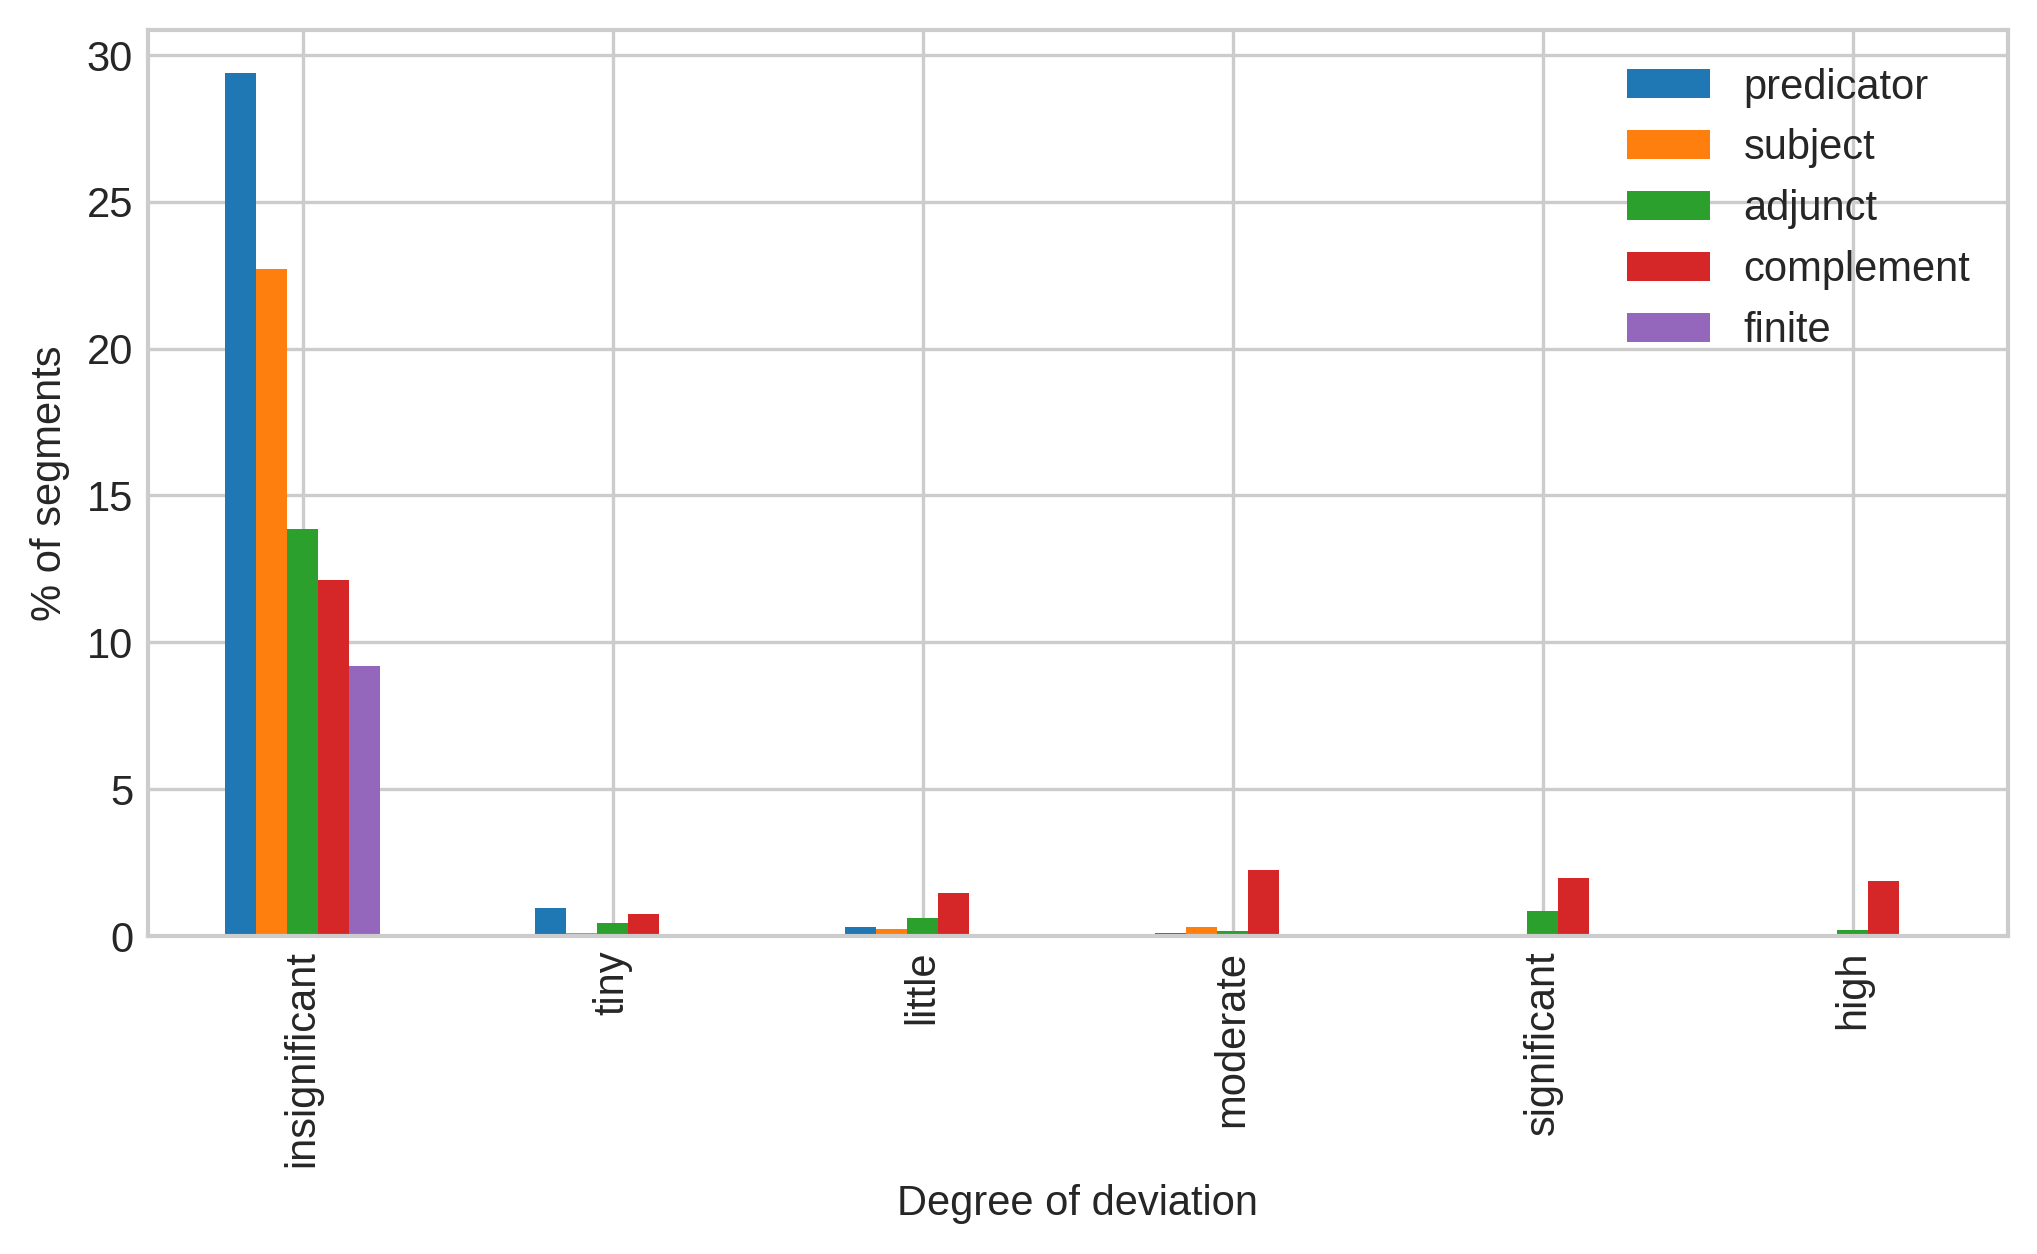
\includegraphics[width=.65\textwidth]{evaluation-results/figures/distance-degree-features-syntactic}
        \caption{Bar chart of the segments deviated to a given degree for major syntactic elements}
        \label{fig:segment-distance-degree-features-mood}
    \end{figure}

    In Figure \ref{fig:segment-distance-degree-features-mood} we can see that most deviations are statistically insignificant. The number of segments in the rest of the bins, from tiny to high, is below 1\% in every bin which perhaps reflects errors in annotation and/or matching algorithm requiring further investigation. In case of complements, however, the proportion of segments is slightly higher (0.7--2.2\%). This may be explained by the problem of prepositional phrase attachment and further analysis is needed to test this hypothesis. 

    When we switch to a grouping by the main Transitivity elements maintaining the same bins defined in Table \ref{tab:progressive-bins}, then the distribution of segment deviations looks as outlined in Table \ref{tab:deviation-per-feature-and-degree-trans}. The same data are depicted in Figure \ref{fig:segment-distance-degree-features-trans}. 

    \begin{table}[!ht]
        \resizebox{0.98\linewidth}{!}{%
        \begin{tabular}{|c|c|c|c|c|c|c|}
            \hline
            \multirow{2}{*}{\textbf{feature}} & \multicolumn{6}{c|}{\textbf{\% of segments per degree of deviation }}                                                                                                                                                 \\ \cline{2-7} 
            & \textbf{\begin{tabular}[c]{@{}c@{}}insignificant\\ (0-3)\end{tabular}} & \textbf{\begin{tabular}[c]{@{}c@{}}tiny\\ (3-5)\end{tabular}} & \textbf{\begin{tabular}[c]{@{}c@{}}little\\ (5-10)\end{tabular}} & \textbf{\begin{tabular}[c]{@{}c@{}}moderate\\ (10-20)\end{tabular}} & \textbf{\begin{tabular}[c]{@{}c@{}}significant\\ (20-50)\end{tabular}} & \textbf{\begin{tabular}[c]{@{}c@{}}high\\ (50-250)\end{tabular}} \\ \hline
            participant-role & 36.78 & 2.21 & 3.48 & 2.80 & 3.04 & 1.67 \\ \hline
            main             & 20.75 & 3.48 & 1.23 & 0.39 & 0.00 & 0.00 \\ \hline
            configuration    & 7.75  & 3.73 & 2.80 & 3.04 & 4.56 & 2.31 \\ \hline
        \end{tabular}
        }
        \caption{Percentage of segments deviated to a given degree for major semantic elements}
        \label{tab:deviation-per-feature-and-degree-trans}
    \end{table}

    \begin{figure}[!ht]
        \centering
        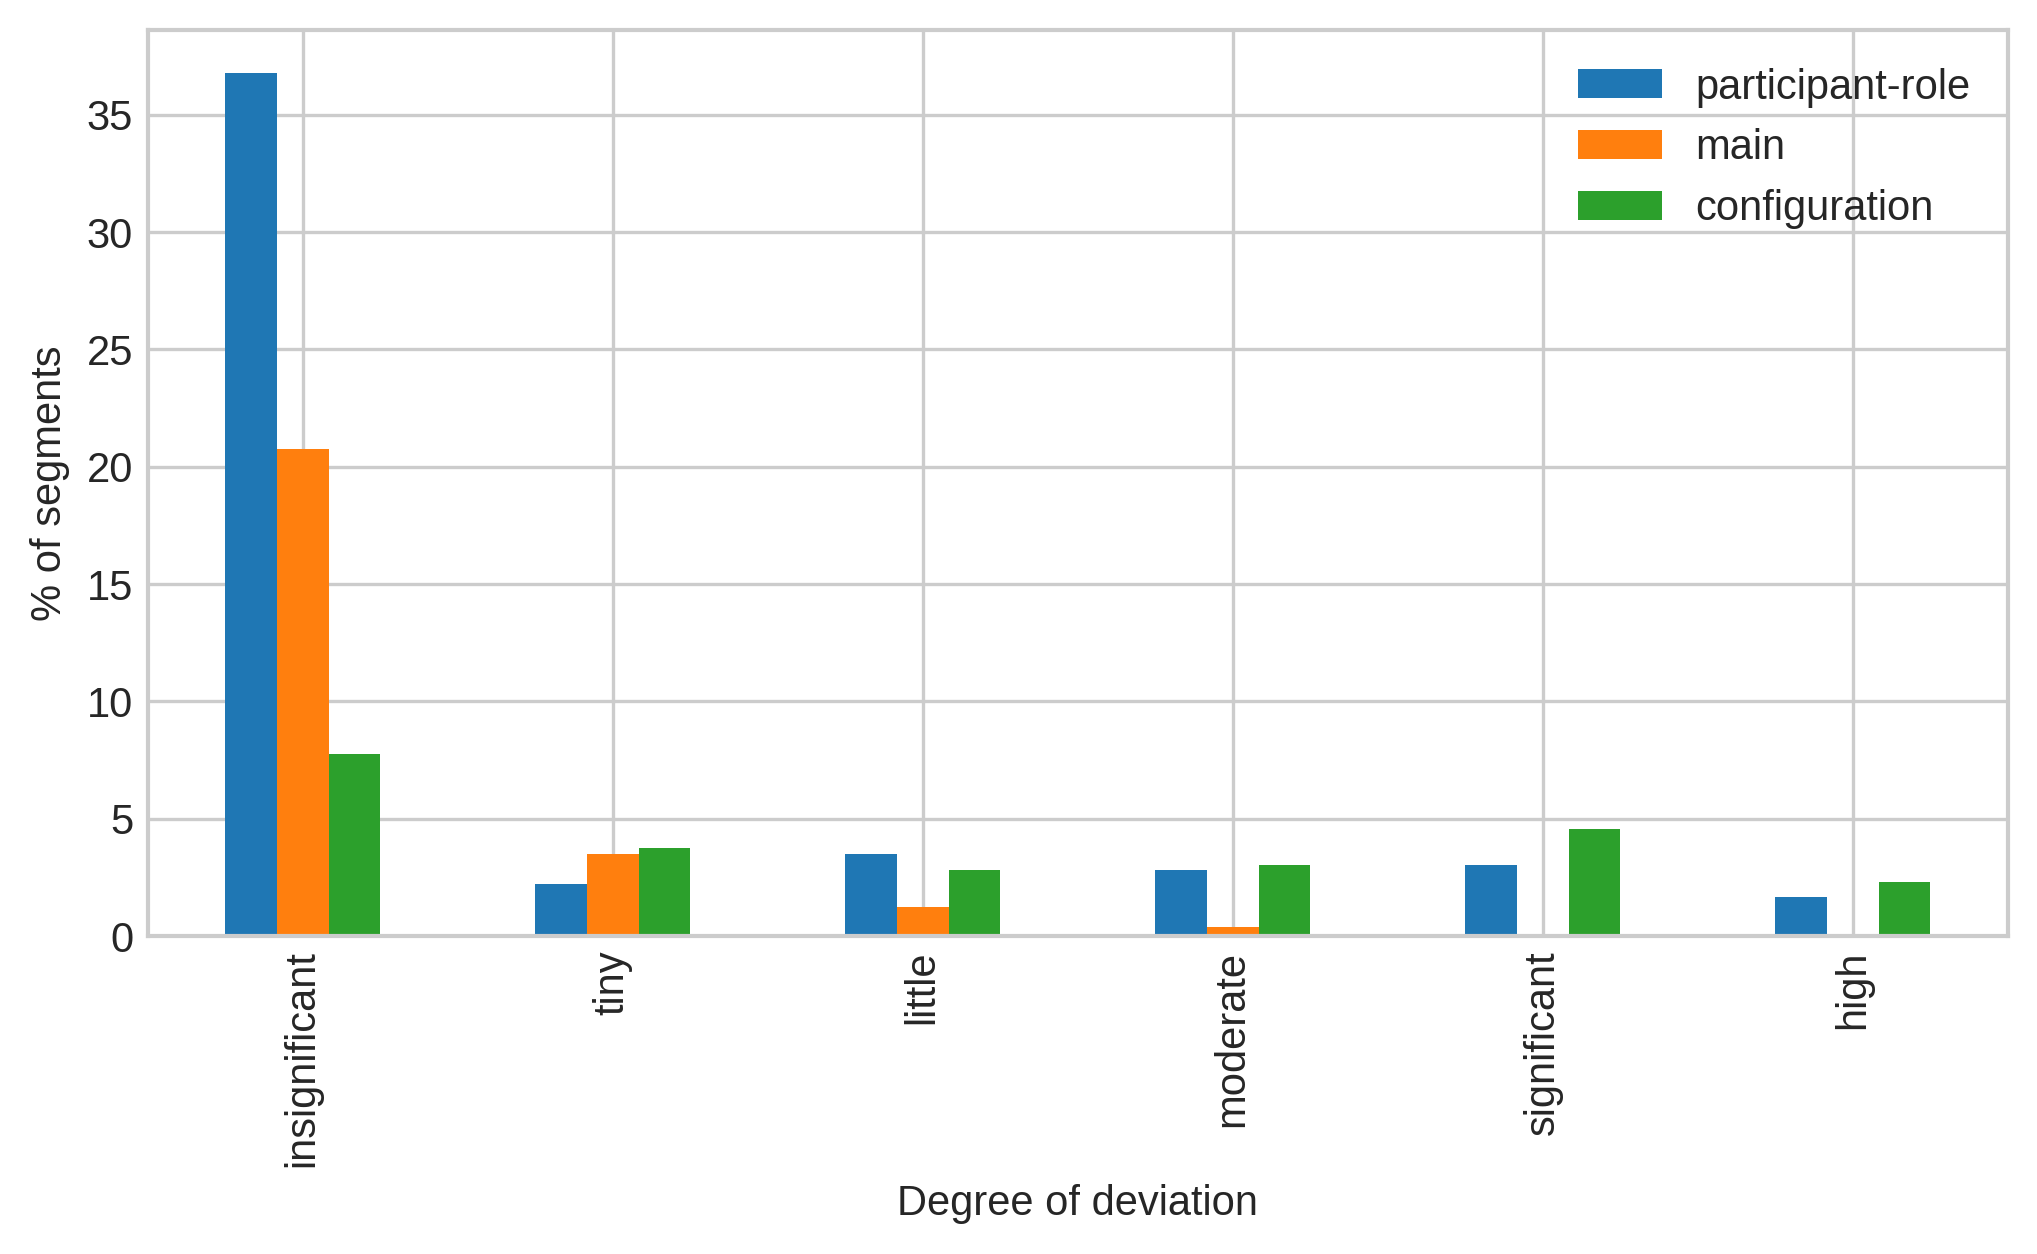
\includegraphics[width=.65\textwidth]{evaluation-results/figures/distance-degree-features-semantic}
        \caption{Bar chart of the feature segments deviated to a given degree for major semantic elements}
        \label{fig:segment-distance-degree-features-trans}
    \end{figure}

    Similarly to Figure \ref{fig:segment-distance-degree-features-mood}, in Figure \ref{fig:segment-distance-degree-features-trans} we can see that most of the deviations are insignificant (0-3 characters). In the rest of the bins representing higher degrees of deviation the amount of segments is up to 4.7\% which reflects higher number of shifted segments. One exception is the main verb whose occurrences decreases towards higher degrees of deviation, i.e. it is shifted by an insignificant, tiny or little degree that is up to about 10 characters. This is explainable by the fact that the main verb is most of the time (if not always) a single word, which is always shorter than the configuration or participant elements which usually span clauses of groups comprising multiple words. The large variations in participant seems to correlate with complement variation and might be explained by the attachment errors. In cases of high configuration deviation however further investigation are needed because these may possibly be errors in the segment matching algorithm or other unknown anomalies.

\subsection{Syntactic evaluation: constituency elements}
\label{sec:syntactic-constituents}
    The evaluation data in this and the following sections will be presented in tables with the same structure. Using Table \ref{tab:constit-unit-types} as example I explain next what the columns mean. The first column will contain the name of the unit type, element or feature. The next three columns \textit{Match}, \textit{Manual mn} and \textit{Parse mn} represent the number of segments that are considered identical between the corpus and parser, the number of unmatched corpus (manually created) segments and the number of unmatched parser (automatically generated) segments. The next three columns \textit{Precision}, \textit{Recall} and \textit{F_1} represent standard accuracy metrics indicating the fraction of relevant instances among the retrieved instances, the fraction of relevant instances that have been retrieved over the total amount of relevant instances and the harmonic mean of the previous two. In addition, the column \textit{\%Total matched} represents the percentage of the current item (row) in the table while the \textit{\% Manual nm} and \textit{\%Parse nm} represent the number of remaining unmatched segments of the current item (row) that represents a translation of the Manual and Parse mn columns into relative terms. 

\begin{table}[!ht]
    \resizebox{\textwidth}{!}{%
        \begin{tabular}{|c|c|c|c|c|c|c|c|c|c|}
            \hline
            \textbf{Unit type} & \textbf{Matched} & \textbf{\begin{tabular}[c]{@{}c@{}}Manual \\ nm\end{tabular}} & \textbf{\begin{tabular}[c]{@{}c@{}}Parse \\ nm\end{tabular}} & \textbf{Precision} & \textbf{Recall} & \textbf{F1} & \textbf{\begin{tabular}[c]{@{}c@{}}\%Total \\ matched\end{tabular}} & \textbf{\begin{tabular}[c]{@{}c@{}}\%Manual \\ nm\end{tabular}} & \textbf{\begin{tabular}[c]{@{}c@{}}\%Parse \\ nm\end{tabular}} \\ \hline
            clause              & 612.00 & 64.00  & 78.00  & 0.89 & 0.91 & 0.90 & 37.00 & 9.47  & 11.30 \\ \hline
            nominal group       & 717.00 & 108.00 & 67.00  & 0.91 & 0.87 & 0.89 & 43.35 & 13.09 & 8.55  \\ \hline
            prepositional group & 119.00 & 39.00  & 39.00  & 0.75 & 0.75 & 0.75 & 7.19  & 24.68 & 24.68 \\ \hline
            adverbial group     & 161.00 & 79.00  & 103.00 & 0.61 & 0.67 & 0.64 & 9.73  & 32.92 & 39.02 \\ \hline
            adjectival group    & 45.00  & 36.00  & 38.00  & 0.54 & 0.56 & 0.55 & 2.72  & 44.44 & 45.78 \\ \hline
        \end{tabular}
    }
    \caption{The evaluation statistics for the main constituency unit types}
    \label{tab:constit-unit-types}
\end{table}

    The syntactic accuracy aims to measure how well the main unit types and the clause main elements have been detected by the parser compared to the corpus. The evaluation is performed on the OCD corpus. This evaluation is restricted to the clause and four group types: nominal, prepositional, adverbial and adjectival. No clause complexes, group complexes or word types are included. The evaluation results are presented in Table \ref{tab:constit-unit-types} where we can see that clauses and nominal groups have an F_1 score of about 90\%. Prepositional, adverbial and adjectival group scores decrease to 55\% and requires investigation of the errors in the parsing and matching algorithms. There is also a contrast in the number of segments, visible in the bar chart from Figure \ref{fig:constit-unit-types}, between the first two element types and the last three with a ratio of one to four or more.

    \begin{figure}[!ht]
        \centering
        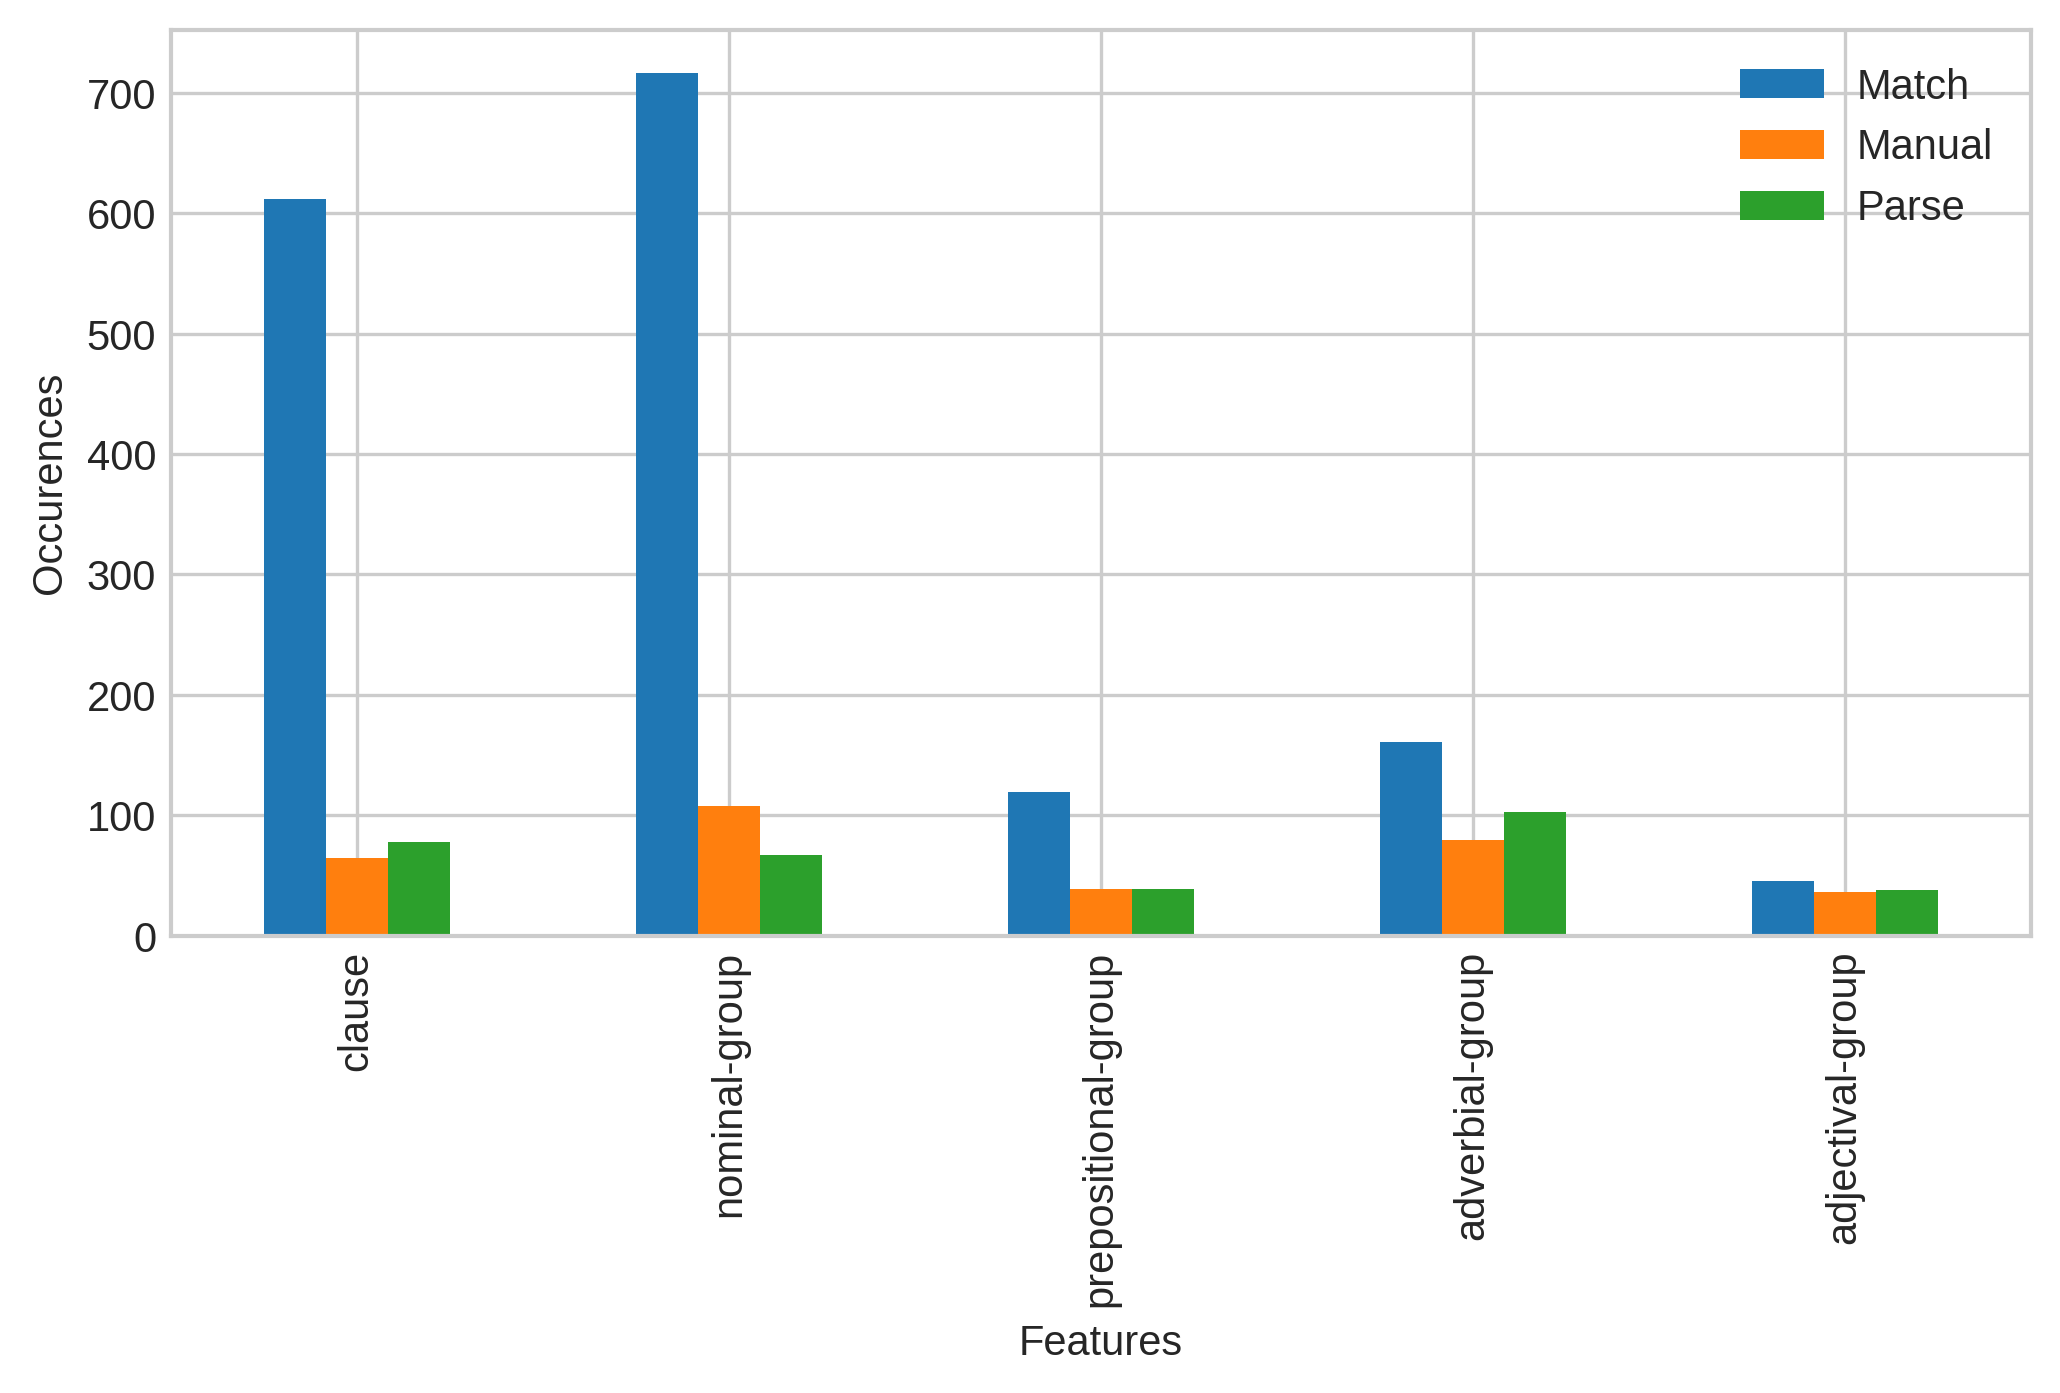
\includegraphics[width=.65\textwidth]{evaluation-results/figures/accuracy-syntactic-group-types}
        \caption{Bar chart of matched and non-matched (manual and parse) segments of the main constituency unit types}
        \label{fig:constit-unit-types}
    \end{figure}

    Table \ref{tab:constit-unit-elements} presents the evaluation result for the main clause elements. Some of them, such as Auxiliary verbs, Main verb extension, Negation particle, and others have been omitted in the corpus and are thus missing in the present evaluation. For the Main verb and Subject elements the F_1 measure raises to 90\%. For the complements and finite the F_1 score is 67\% and 63\%. Surprisingly, the Complements have a small number of corpus unmatched segments and a high number of parser unmatched segments. This is explained by a flaw in the annotation methodology because the clausal complements were often annotated directly as new clause and omitting to draw the same segment with complement element. This required the corpus revision and correction. Adjuncts however have a higher number of unmatched segments on both sides and this may be due to bugs in the parser.

    \begin{table}[!ht]
        \resizebox{\textwidth}{!}{%
            \begin{tabular}{|c|c|c|c|c|c|c|c|c|c|}
                \hline
                \textbf{Element} & \textbf{Matched} & \textbf{\begin{tabular}[c]{@{}c@{}}Manual \\ nm\end{tabular}} & \textbf{\begin{tabular}[c]{@{}c@{}}Parse \\ nm\end{tabular}} & \textbf{Precision} & \textbf{Recall} & \textbf{F1} & \textbf{\begin{tabular}[c]{@{}c@{}}\%Total \\ matched\end{tabular}} & \textbf{\begin{tabular}[c]{@{}c@{}}\%Manual \\ nm\end{tabular}} & \textbf{\begin{tabular}[c]{@{}c@{}}\%Parse \\ nm\end{tabular}} \\ \hline
                Main verb & 613 & 60  & 79  & 0.89 & 0.91 & 0.90 & 30.79 & 8.92  & 11.42 \\ \hline
                Subject    & 466 & 22  & 86  & 0.84 & 0.95 & 0.90 & 23.41 & 4.51  & 15.58 \\ \hline
                Complement & 406 & 43  & 350 & 0.54 & 0.90 & 0.67 & 20.39 & 9.58  & 46.30 \\ \hline
                Adjunct    & 321 & 159 & 224 & 0.59 & 0.67 & 0.63 & 16.12 & 33.12 & 41.10 \\ \hline
                Finite     & 185 & 3   & 392 & 0.32 & 0.98 & 0.48 & 9.29  & 1.60  & 67.94 \\ \hline
            \end{tabular}
        }
        \caption{The evaluation statistics for the clause main elements}
        \label{tab:constit-unit-elements}
    \end{table}

    \begin{figure}[!ht]
        \centering
        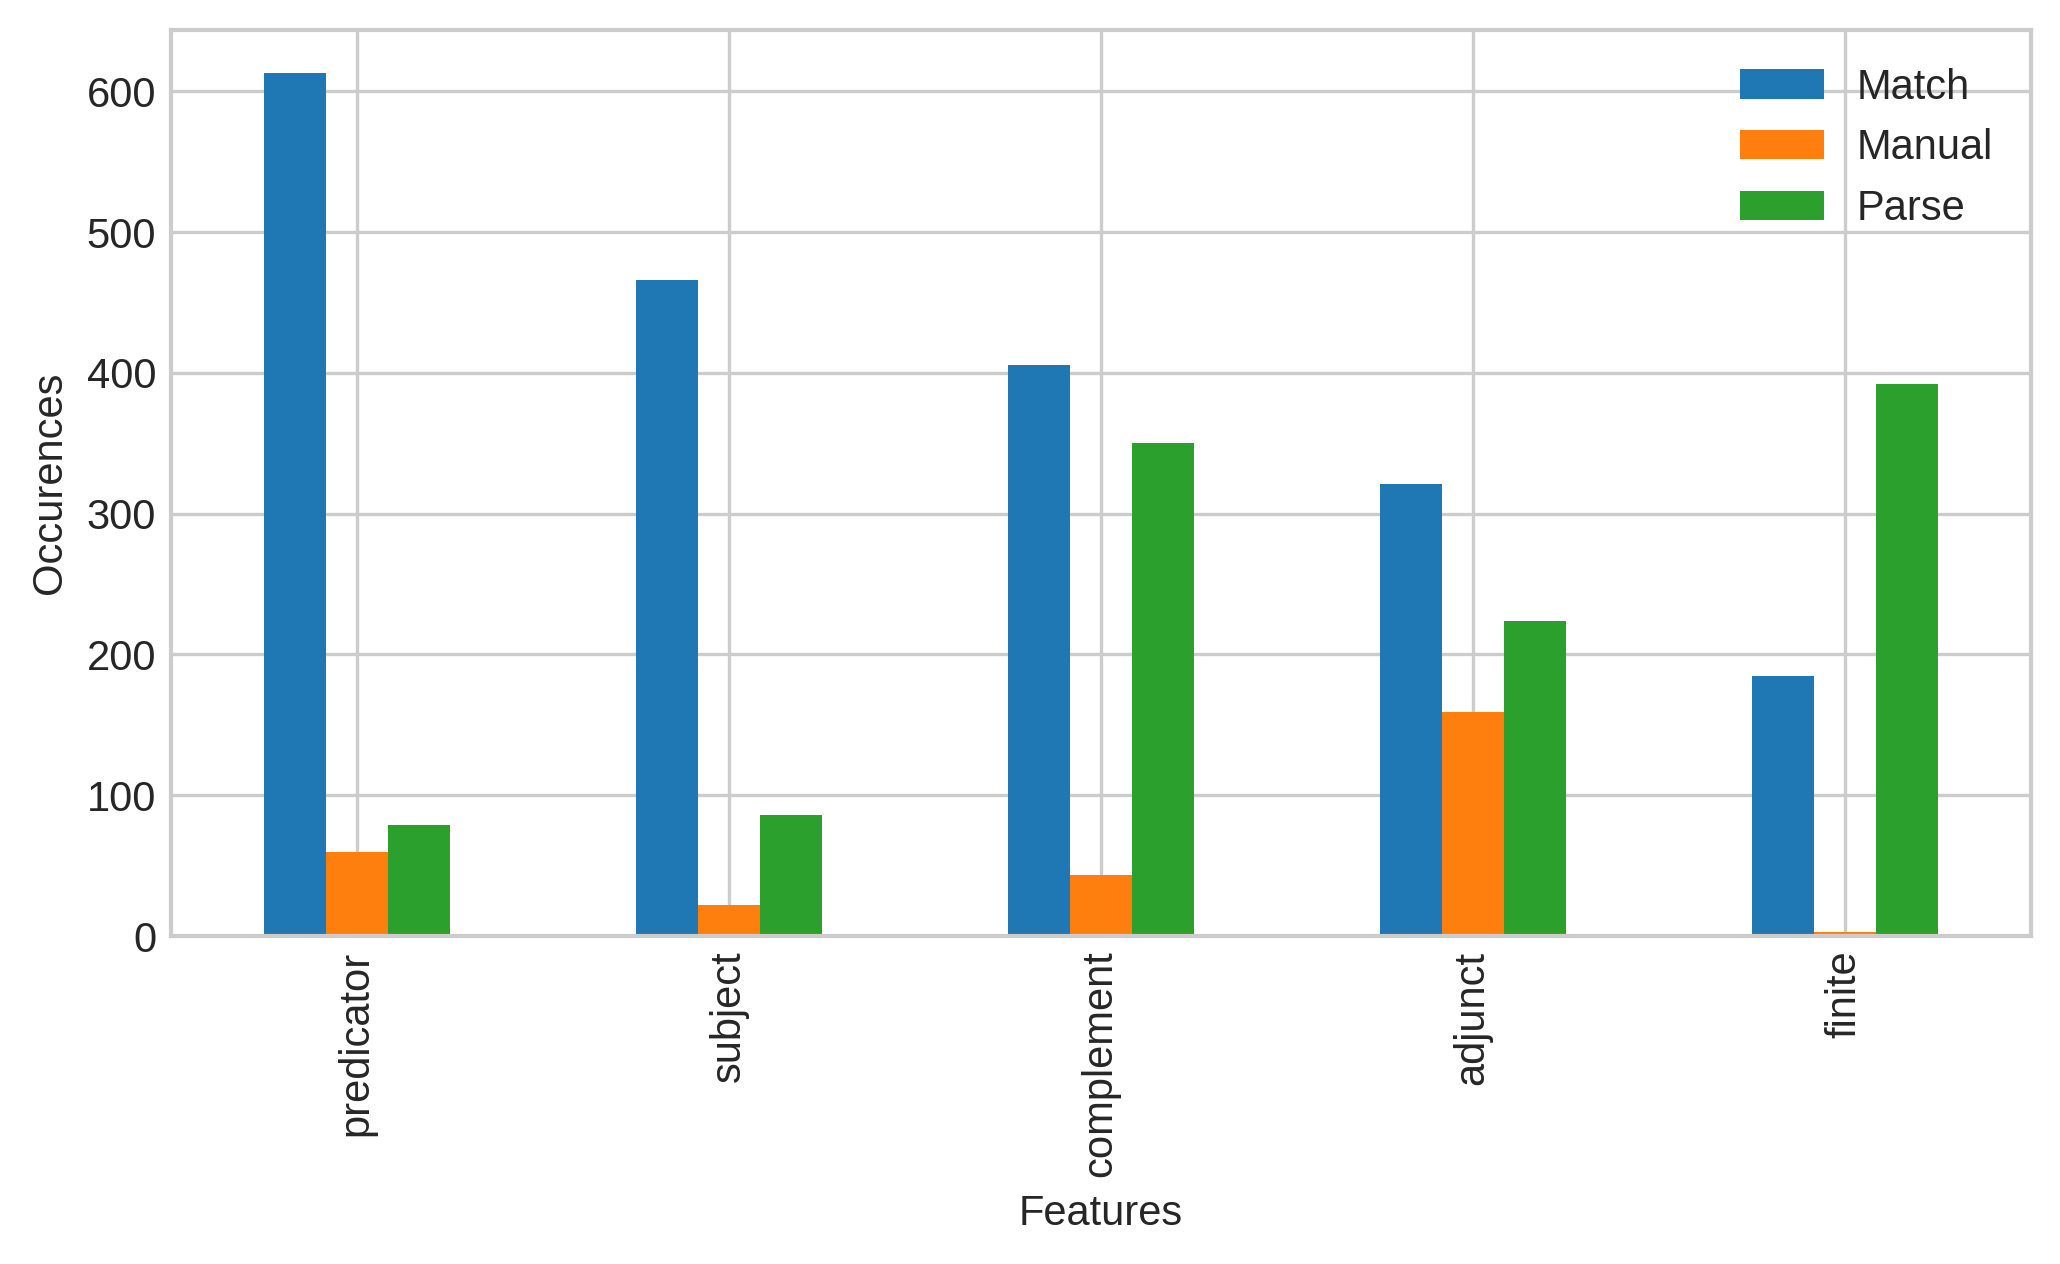
\includegraphics[width=.65\textwidth]{evaluation-results/figures/accuracy-syntactic-clause-elements}
        \caption{Bar chart of matched and non-matched (manual and parse) segments of the clause main elements}
        \label{fig:constit-unit-elements}
    \end{figure}

\subsection{Syntactic evaluation: MOOD features}
\label{sec:syntactic-features}
    In this section I present the evaluation of the MOOD system network selections. The corpus contains selections from a part of the system network that is depicted in Figure \ref{fig:mood-ocd-simplified}. The full system network is provided in Figure \ref{fig:clause-mood}. Employing the entire system network in the annotations was difficult because as the delicacy increases the time spent for the annotation process increases. 

    \begin{figure}[!ht]
        \centering
        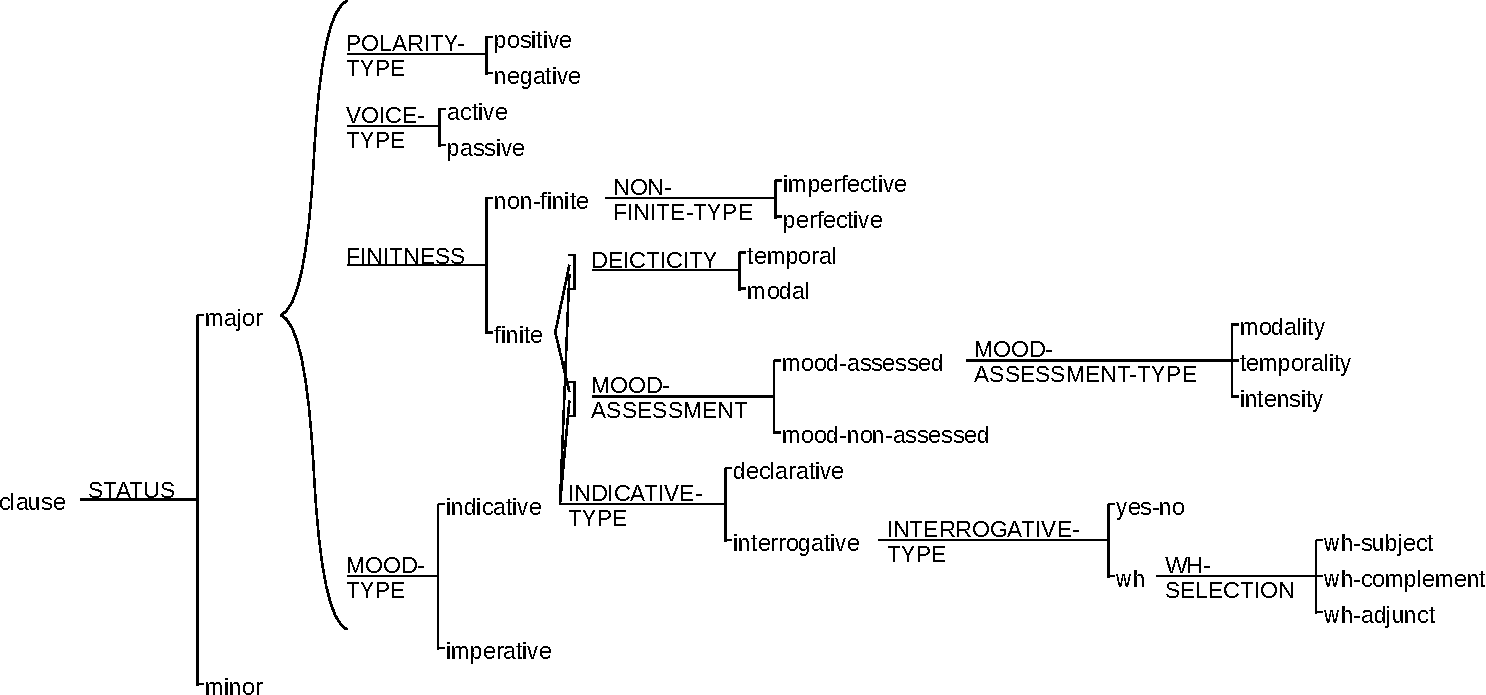
\includegraphics[width=.65\textwidth]{Figures/Evaluation/ocd1-mood-simplified.pdf}
        \caption{The part of the MOOD system network that has been used in OCD corpus annotation}
        \label{fig:mood-ocd-simplified}
    \end{figure}

    \begin{table}[!ht]
        \resizebox{\textwidth}{!}{%
            \begin{tabular}{|c|c|c|c|c|c|c|c|c|c|}
                \hline
                \textbf{Feature} & \textbf{Matched} & \textbf{\begin{tabular}[c]{@{}c@{}}Manual \\ nm\end{tabular}} & \textbf{\begin{tabular}[c]{@{}c@{}}Parse \\ nm\end{tabular}} & \textbf{Precision} & \textbf{Recall} & \textbf{F1} & \textbf{\begin{tabular}[c]{@{}c@{}}\%Total \\ matched\end{tabular}} & \textbf{\begin{tabular}[c]{@{}c@{}}\%Manual \\ nm\end{tabular}} & \textbf{\begin{tabular}[c]{@{}c@{}}\%Parse \\ nm\end{tabular}} \\ \hline
                POLARITY-TYPE &  &  &  &  &  &  &  &  &  \\ \hline
                positive & 485 & 125 & 55 & 0.90 & 0.80 & 0.84 & 89.48 & 20.49 & 10.19 \\ \hline
                negative & 57  & 10  & 70 & 0.45 & 0.85 & 0.59 & 10.52 & 14.93 & 55.12 \\ \hline
                VOICE-TYPE &  &  &  &  &  &  &  &  &  \\ \hline
                active  & 553 & 102 & 68 & 0.89 & 0.84 & 0.87 & 98.05 & 15.57 & 10.95 \\ \hline
                passive & 11  & 11  & 28 & 0.28 & 0.50 & 0.36 & 1.95  & 50.00 & 71.79 \\ \hline
                FINITNESS &  &  &  &  &  &  &  &  &  \\ \hline
                non-finite   & 99  & 19 & 38  & 0.72 & 0.84 & 0.78 & 15.84 & 16.10 & 27.74 \\ \hline
                finite       & 526 & 33 & 554 & 0.49 & 0.94 & 0.64 & 84.16 & 5.90  & 51.30 \\ \hline
                NON-FINITE-TYPE &  &  &  &  &  &  &  &  &  \\ \hline
                perfective   & 71  & 12 & 16  & 0.82 & 0.86 & 0.84 & 73.20 & 14.46 & 18.39 \\ \hline
                imperfective & 26  & 9  & 24  & 0.52 & 0.74 & 0.61 & 26.80 & 25.71 & 48.00 \\ \hline
                DEICTICITY &  &  &  &  &  &  &  &  &  \\ \hline            
                temporal & 446 & 74 & 55 & 0.89 & 0.86 & 0.87 & 97.38 & 14.23 & 10.98 \\ \hline
                modal    & 12  & 33 & 6  & 0.67 & 0.27 & 0.38 & 2.62  & 73.33 & 33.33 \\ \hline
                MOOD-ASSESSMENT-TYPE  &  &  &  &  &  &  &  &  &  \\ \hline            
                temporality & 35 & 17 & 27 & 0.56 & 0.67 & 0.61 & 56.45 & 32.69 & 43.55 \\ \hline
                modality    & 15 & 32 & 8  & 0.65 & 0.32 & 0.43 & 24.19 & 68.09 & 34.78 \\ \hline
                intensity   & 12 & 14 & 43 & 0.22 & 0.46 & 0.30 & 19.35 & 53.85 & 78.18 \\ \hline
                MOOD-TYPE  &  &  &  &  &  &  &  &  &  \\ \hline                        
                indicative    & 455 & 216 & 37 & 0.92 & 0.68 & 0.78 & 99.13 & 32.19 & 7.52  \\ \hline
                imperative    & 4   & 1   & 31 & 0.11 & 0.80 & 0.20 & 0.87  & 20.00 & 88.57 \\ \hline
                INDICATIVE-TYPE  &  &  &  &  &  &  &  &  &  \\ \hline                        
                declarative   & 355 & 260 & 27 & 0.93 & 0.58 & 0.71 & 88.31 & 42.28 & 7.07  \\ \hline
                interrogative & 47  & 7   & 63 & 0.43 & 0.87 & 0.57 & 11.69 & 12.96 & 57.27 \\ \hline
                INTERROGATIVE-TYPE  &  &  &  &  &  &  &  &  &  \\ \hline   
                 wh            & 40  & 6   & 57 & 0.41 & 0.87 & 0.56 & 88.89 & 13.04 & 58.76 \\ \hline
                yes-no        & 5   & 3   & 8  & 0.38 & 0.62 & 0.48 & 11.11 & 37.50 & 61.54 \\ \hline                     
                WH-SELECTION  &  &  &  &  &  &  &  &  &  \\ \hline                        
                wh-subject    & 9   & 3   & 7  & 0.56 & 0.75 & 0.64 & 32.14 & 25.00 & 43.75 \\ \hline
                wh-adjunct    & 11  & 15  & 3  & 0.79 & 0.42 & 0.55 & 39.29 & 57.69 & 21.43 \\ \hline
                wh-complement & 8   & 0   & 62 & 0.11 & 1.00 & 0.21 & 28.57 & 0.00  & 88.57 \\ \hline
            \end{tabular}
        }
        \caption{The evaluation statistics available for the MOOD system network}
        \label{tab:features-mood}
    \end{table}

    Table \ref{tab:features-mood} summarises the evaluation results for the MOOD system network features grouped by system names (in capitals). The precision and recall values vary quite a lot from a minimum of 11\% up to a maximum of 93\% and the harmonic mean, the F_1 score, between 30\% up to 87\%  averaging to almost 60\%. The details can be read in Table \ref{tab:mood-accuracy}. The distribution of these values can be seen in Figures \ref{fig:mood-precission-recall} and \ref{fig:mood-precission-f1}. A noticeable feature is the presence of two peaks in the precision and recall distributions: one around 50\% and the other one around 90\%. They translate into a similar F_1 distribution with peaks at 60\% and 85\%.

    \begin{table}[!ht]
        \centering
        \begin{tabular}{|c|c|c|c|}
            \hline
            \textbf{} & \textbf{precision} & \textbf{recall} & \textbf{F1} \\ \hline
            feature count & 21.00 & 21.00 & 21.00 \\ \hline
            mean & 0.57 & 0.73 & 0.59 \\ \hline
            standard deviation & 0.27 & 0.18 & 0.21 \\ \hline
            min value & 0.11 & 0.32 & 0.20 \\ \hline
            25\% quantile & 0.41 & 0.62 & 0.48 \\ \hline
            50\% quantile & 0.56 & 0.80 & 0.61 \\ \hline
            75\% quantile & 0.82 & 0.86 & 0.78 \\ \hline
            max value & 0.93 & 1.00 & 0.87 \\ \hline
        \end{tabular}
        \caption{Descriptive statistics of the precision, recall and F1 scores}
        \label{tab:mood-accuracy}
    \end{table}

    \noindent
    \begin{minipage}[t]{0.475\textwidth}
        \centering
        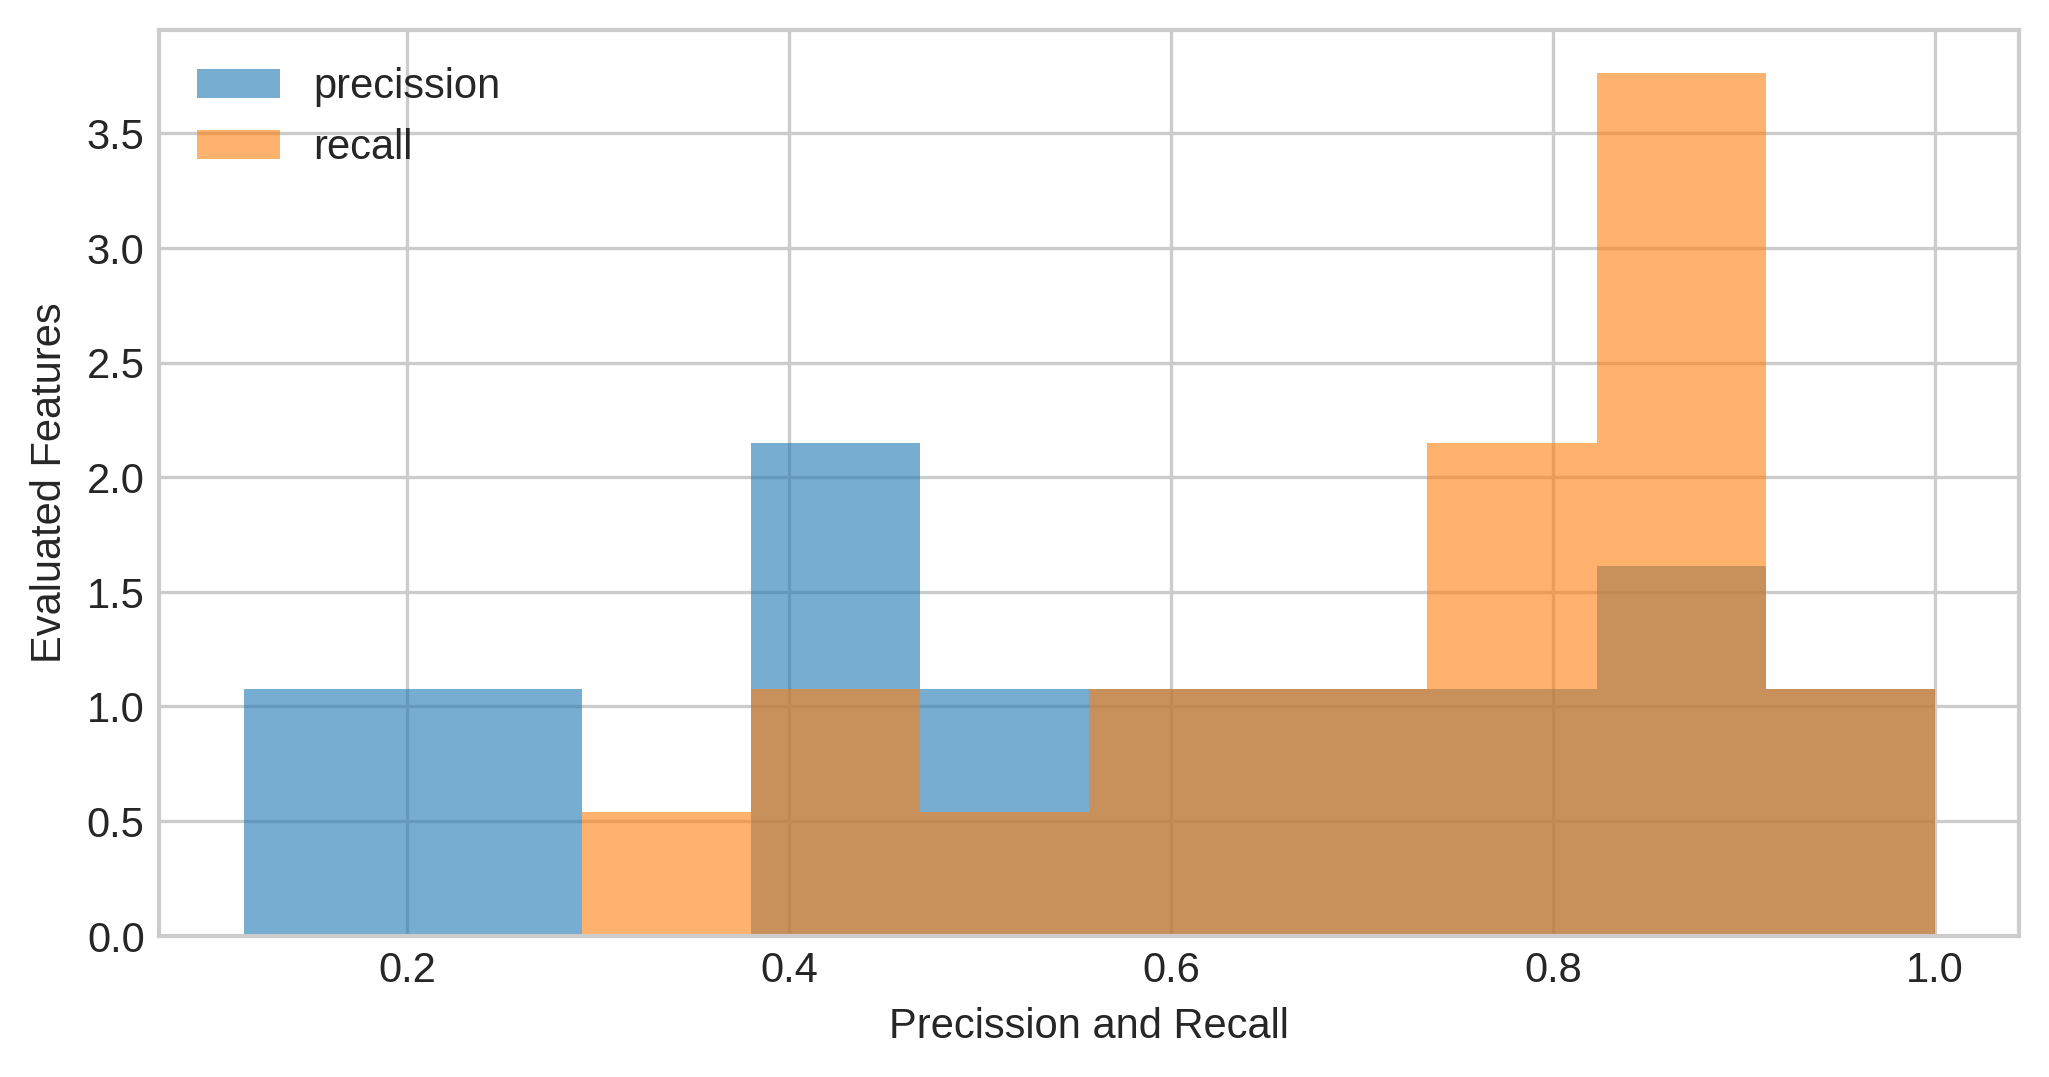
\includegraphics[width=\textwidth]{evaluation-results/figures/accuracy-syntactic-mood-precission-recall.png}
        \captionof{figure}{The distribution of precision and recall for selected features from the MOOD system network}
        \label{fig:mood-precission-recall}
    \end{minipage}
    \quad
    \begin{minipage}[t]{0.475\textwidth}
        \centering
        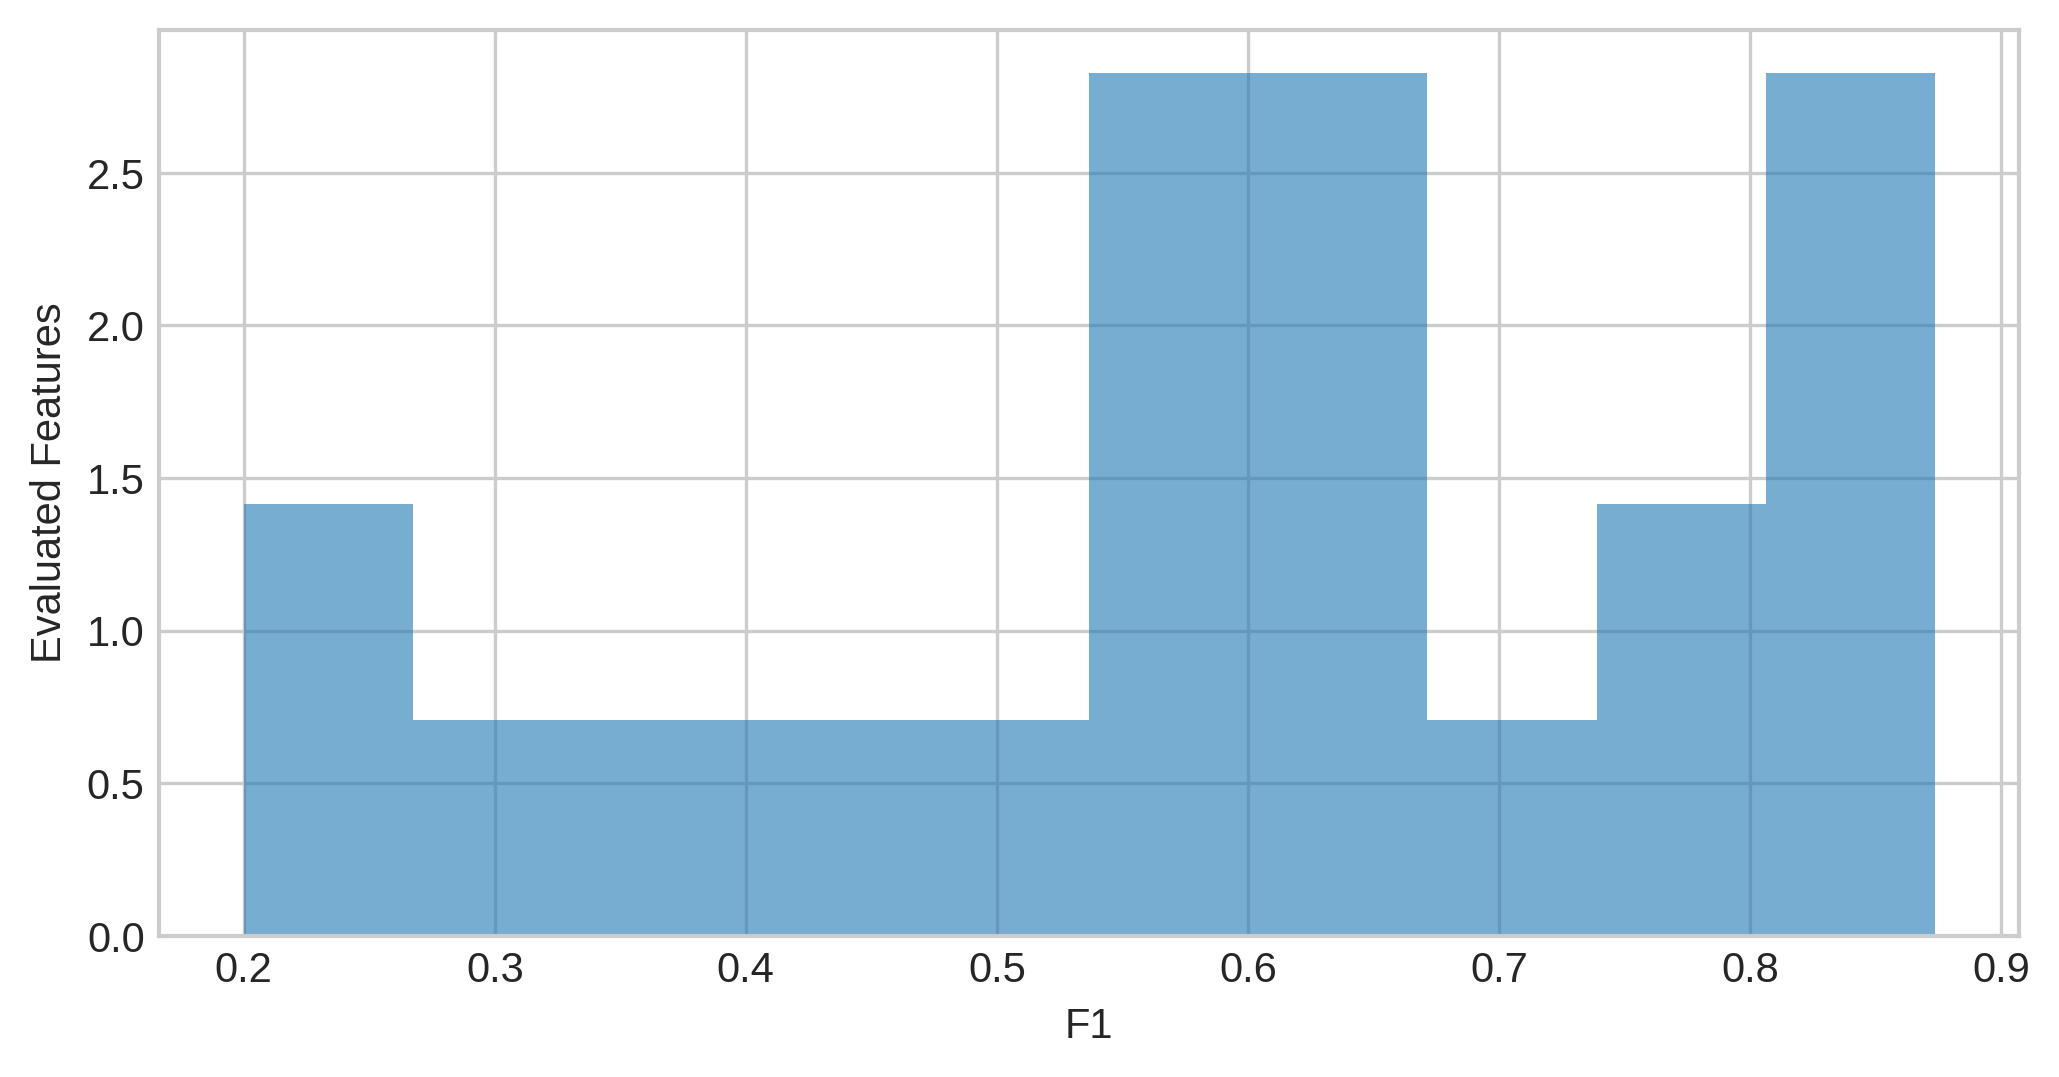
\includegraphics[width=\textwidth]{evaluation-results/figures/accuracy-syntactic-mood-f1.png}
        \captionof{figure}{The distribution of F1 score for selected features from the MOOD system network}
        \label{fig:mood-precission-f1}
    \end{minipage}
    \vspace{1em}

    Within most systems, the F_1 scores exhibit high contrast from one feature to the other. What this means is discussed in the next two cases. For example in the POLARITY-TYPE system the positive polarity feature scores 84\% F_1 measure and negative one almost 60\%. As per Definition \ref{def:system}, the system features are mutually exclusive. The polarity of an English clause is positive by default unless a negation marker is found and this represents only 10\% of the clauses in  the corpus. This means that it should be sufficient for the parser to detect one feature with a reasonably high F_1 score then the converse feature should be detectable with the same degree of accuracy. Yet the current data invalidate this hypothesis. 

    In the case of the POLARITY-TYPE system, the phenomena may be explained as a consequence of low delicacy in the parsing algorithm. The current implementation determines polarity by checking for the presence of the negation verbal marker only. Nonetheless a more delicate polarity testing will have to take into consideration polarity indicators from the subject, complement and adjuncts of various types that may have been taken into consideration during the annotation process. Providing an incomplete, less delicate implementation for systemic choices may be a source of errors. This hypothesis requires further investigation.  %The same can be expected of other systems that are reduced in delicacy 

    Nonetheless, the same phenomena can be seen if we look at the systems that do not span others with higher degrees of delicacy. For example, the detection mechanism for VOICE-TYPE is implemented similarly to POLARITY-TYPE. The parser checks whether there is a passive order of elements in the clause, otherwise the active voice is selected.  Detection of the positive voice scores a much higher F_1 measure of 87\% than the negative one of 36\%. There is no problem of low delicacy and still there is a discrepancy between the F_1 scores of the two features. %which is somehow counter intuitive result.  

    %This interpretation however is not entirely correct and there is another way of looking at this discrepancy. 
    This high discrepancy between the feature F_1 scores can be seen as follows. Most instances of active voice are easy to detect. But there is a portion of cases, regardless of the voice, that are difficult for the parser to distinguish. The passive voice selections are executed mostly for these ambiguous cases. More investigation is required to pinpoint exactly how such phenomena materialise.

    Nonetheless, in future implementations we can take advantage of the mutual exclusivity of system features and capitalise on the above finding, at least for the leaf systems. Taking into consideration that the score of one feature is higher, clause elements should then be provided with selections of those features only, while the complement features scoring low in this evaluation should remain unassigned. This means that only features that can be provided with high confidence (using F_1 score as a measure of that) shall be assigned. Then an additional process can be implemented to select the remaining unassigned features. 

    %Next I proceed to discuss the semantic features implemented in the parser. 

\subsection{Semantic evaluation: constituency elements}
\label{sec:semantic-constituents}
    This section describes the empirical findings regarding semantic parsing. This evaluation is based on the OE1 and BTC corpora created by Anke Schultz for her PhD project. The text is annotated according to the Cardiff TRANSITIVITY system network. The employed elements are Configuration, Participant role and Main verb while Circumstances are excluded from the study. Table \ref{tab:configuration-elements} summarises the empirical findings. 

    \begin{table}[!ht]
        \resizebox{\textwidth}{!}{%    
        \begin{tabular}{|c|c|c|c|c|c|c|c|c|c|}
            \hline
            \textbf{Element} & \textbf{Match} & \textbf{\begin{tabular}[c]{@{}c@{}}Manual\\ nm\end{tabular}} & \textbf{\begin{tabular}[c]{@{}c@{}}Parse\\ nm\end{tabular}} & \textbf{Precision} & \textbf{Recall} & \textbf{F1} & \textbf{\begin{tabular}[c]{@{}c@{}}\%Total \\ matched\end{tabular}} & \textbf{\begin{tabular}[c]{@{}c@{}}\%Manual\\ nm\end{tabular}} & \textbf{\begin{tabular}[c]{@{}c@{}}\%Parse\\ nm\end{tabular}} \\ \hline
            Participant role & 2780 & 233 & 1002 & 0.74 & 0.92 & 0.82 & 49.54 & 7.73 & 26.49 \\ \hline
            Configuration & 1376 & 127 & 493 & 0.74 & 0.92 & 0.82 & 24.52 & 8.45 & 26.38 \\ \hline
            Main Verb & 1456 & 160 & 605 & 0.71 & 0.90 & 0.79 & 25.94 & 9.90 & 29.35 \\ \hline
        \end{tabular}
        }
        \caption{The evaluation statistics for the main semantic elements}
        \label{tab:configuration-elements}
    \end{table}
    \begin{figure}[!ht]
        \centering
        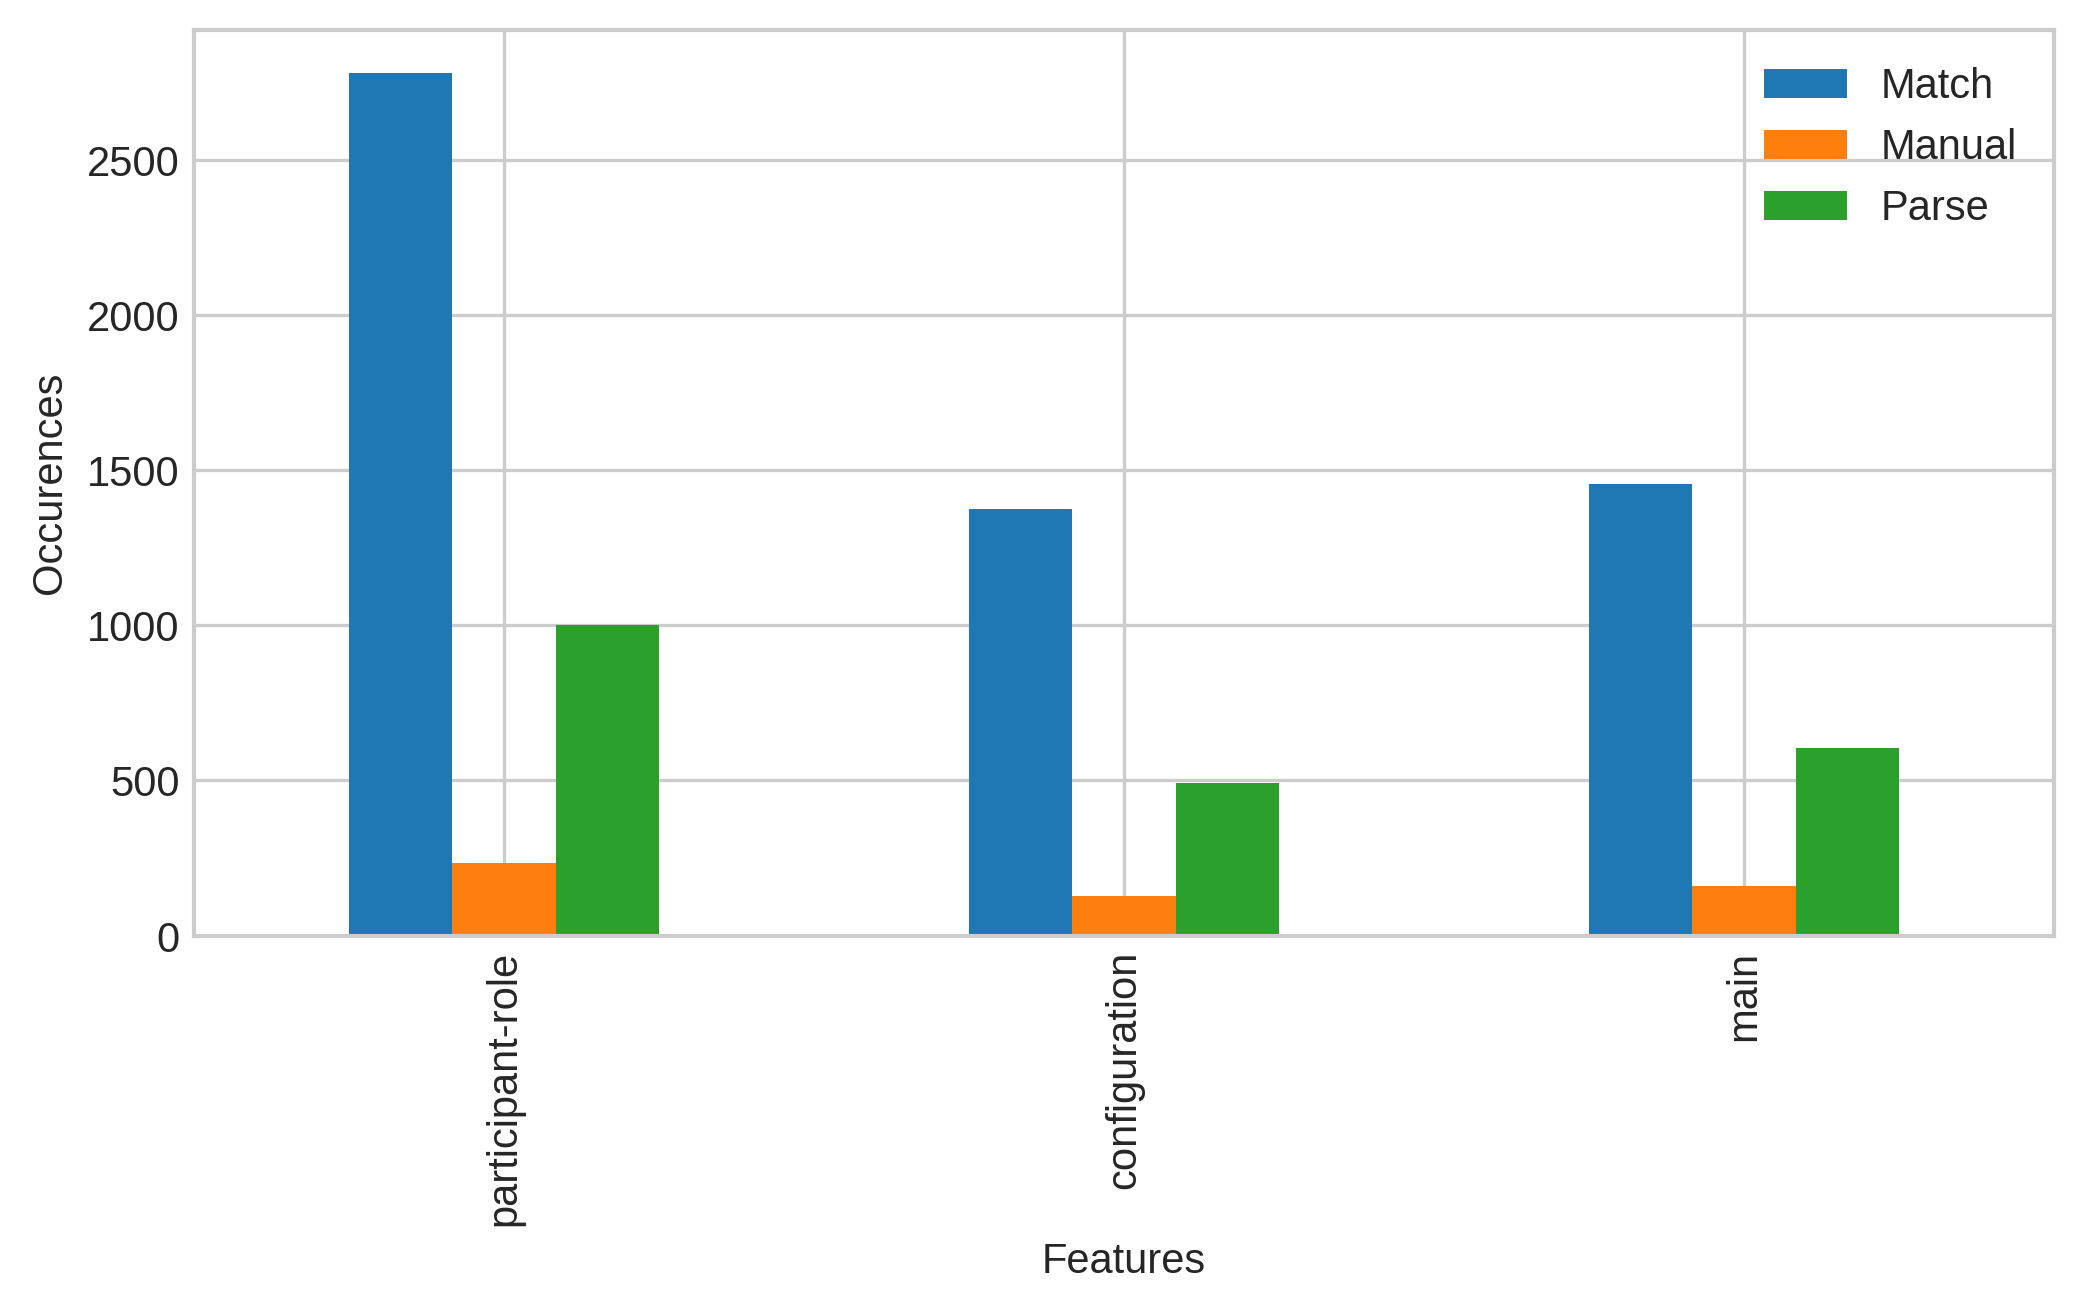
\includegraphics[width=.65\textwidth]{evaluation-results/figures/accuracy-semantic-figure-elements}
        \caption{Bar chart of matched and non-matched (manual and parse) segments of the main semantic elements}
        \label{fig:configuration-elements}
    \end{figure}

    The F_1 score (82\%), precision (74\%) and recall (92\%) vary very little across elements when compared to the same scores for syntactic elements shown in Table \ref{tab:constit-unit-elements} above which vary substantially from one element to another. The score stability of the former may be explained by higher quality of annotation. 

    Another explanation could be the lower granularity of elements. Text segments of Configurations in this case correspond to clause segments, Participant roles to both Subjects and Complements, while the Main verb segments are shared. The aggregation of Subjects and Complements can be observed in Figure \ref{fig:configuration-elements} where the number of participant roles is approximately double the number of configurations under the hypothesis that the average number of participants per clause is close to two. Next I present an analysis of the systemic feature selections data from the TRANSITIVITY system network. 

\subsection{Semantic evaluation: TRANSITIVITY features}
\label{sec:semantic-features}
    In this section I present the evaluation of the TRANSITIVITY system network. The corpus contains annotations with the part from the original system network shown in Figure \ref{fig:cardiff-transitivity}. The limitation is in the number of process types and is represented in Figure \ref{fig:transitivity-simplified}. Employing the entire system network in the annotation process increases in difficulty as the delicacy increases due to the time need to do the job. 

    \begin{figure}[!ht]
        \centering
        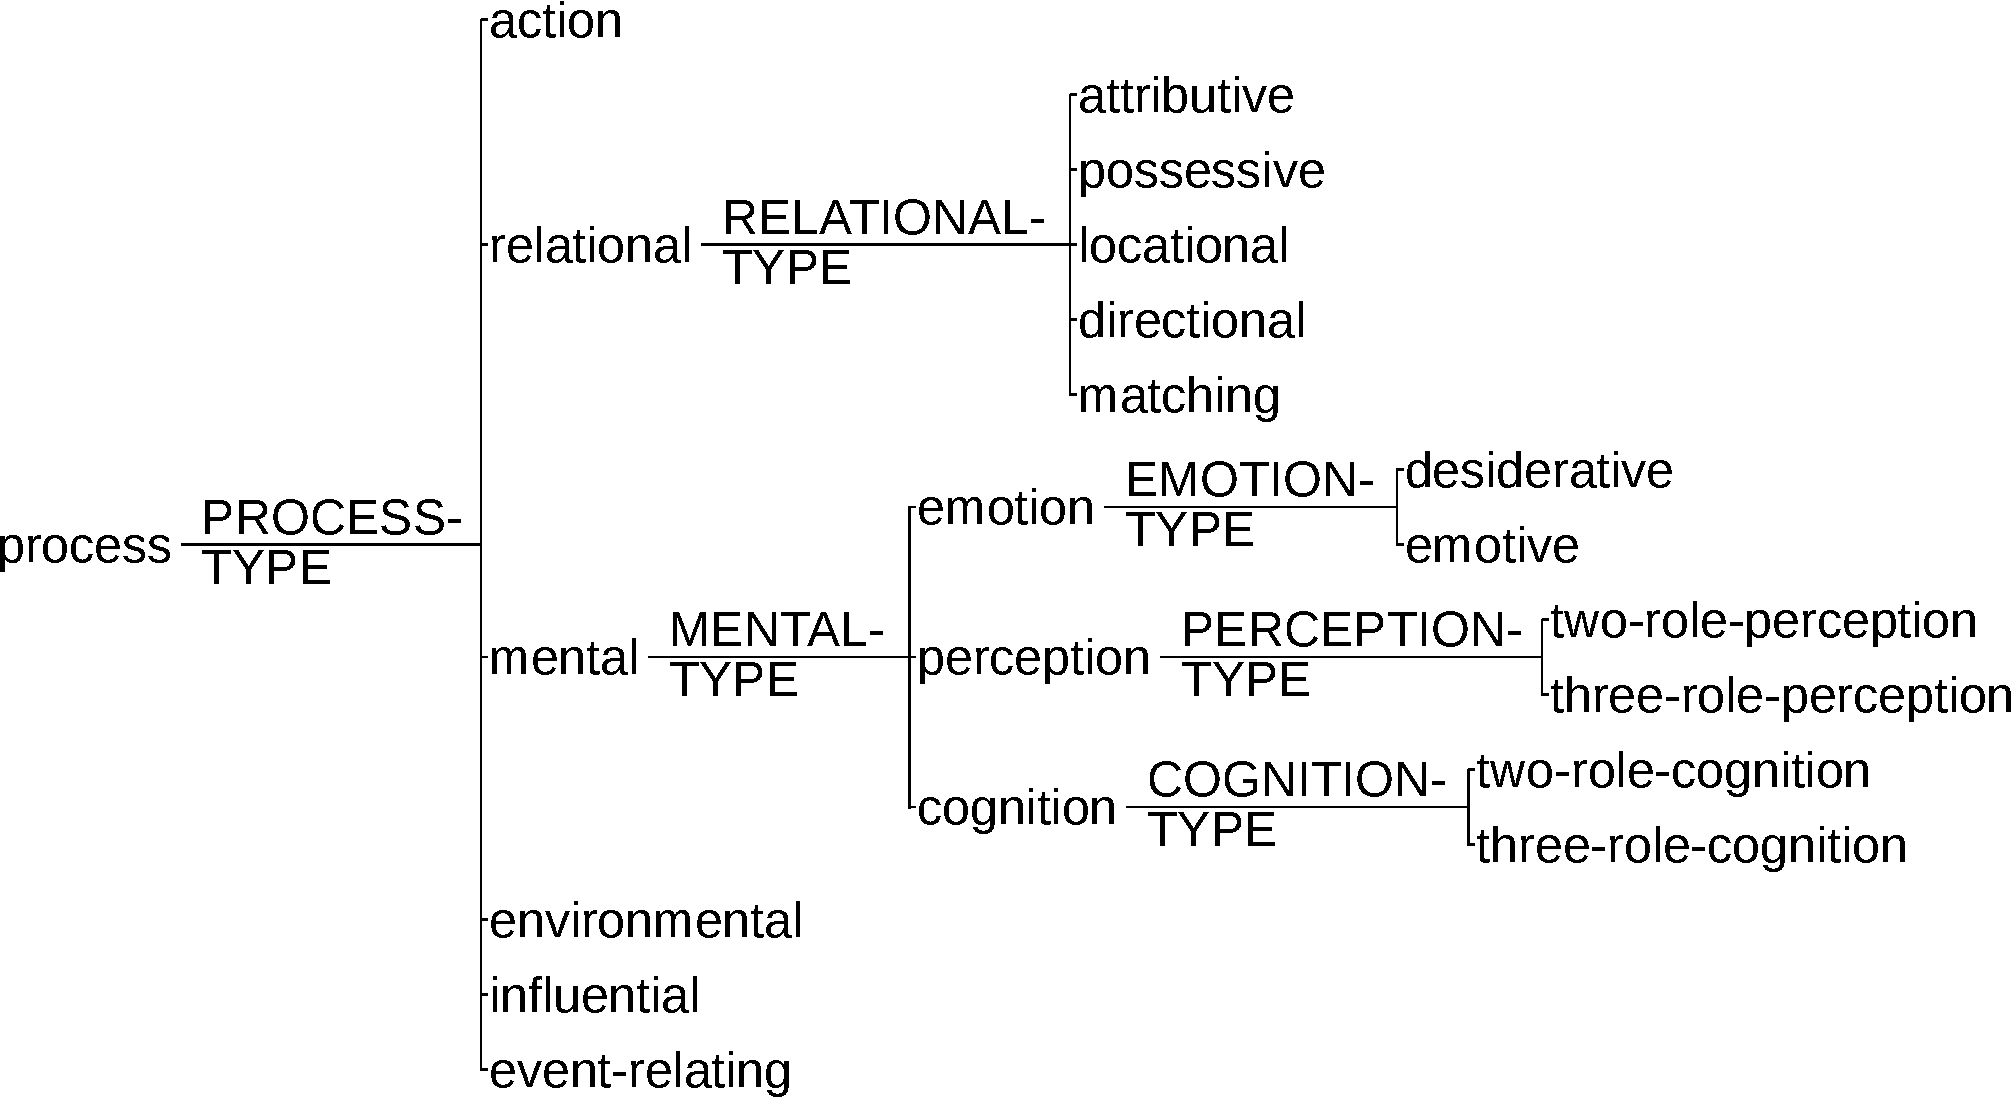
\includegraphics[width=.65\textwidth]{Figures/Evaluation/trans-simplified.pdf}
        \caption{The fragment of the TRANSITIVITY system network that has been used in the corpus}
        \label{fig:transitivity-simplified}
    \end{figure}

    Transitivity analysis is semantic in nature and poses challenges in meaning selection beyond constituent class or function. Unlike other approaches where parser offers the most likely choice from the set of possible ones, the current parser has no means to differentiate between the alternatives and thus provides a set of possible configurations for each clause. Intuitively, this should reduce recall on all the elements but the effects are manifested only at the level of participant roles as will be described below. But first let's discuss the measurements on process types provided in Table \ref{tab:features-transitivity}. 

    \begin{table}[!ht]
        \resizebox{\textwidth}{!}{%  
        \begin{tabular}{|c|c|c|c|c|c|c|c|c|c|}
            \hline
            \textbf{Feature} & \textbf{Match} & \textbf{\begin{tabular}[c]{@{}c@{}}Manual\\ nm\end{tabular}} & \textbf{\begin{tabular}[c]{@{}c@{}}Parse\\ nm\end{tabular}} & \textbf{Precision} & \textbf{Recall} & \textbf{F1} & \textbf{\begin{tabular}[c]{@{}c@{}}\%Total \\ matched\end{tabular}} & \textbf{\begin{tabular}[c]{@{}c@{}}\%Manual\\ nm\end{tabular}} & \textbf{\begin{tabular}[c]{@{}c@{}}\%Parse\\ nm\end{tabular}} \\ \hline
            PROCESS-TYPE &  &  &  &  &  &  &  &  &  \\ \hline
            mental & 277 & 231 & 87 & 0.76 & 0.55 & 0.64 & 33.62 & 45.47 & 23.90 \\ \hline
            relational & 338 & 297 & 174 & 0.66 & 0.53 & 0.59 & 41.02 & 46.77 & 33.98 \\ \hline
            influential & 38 & 51 & 62 & 0.38 & 0.43 & 0.40 & 4.61 & 57.30 & 62.00 \\ \hline
            action & 170 & 231 & 352 & 0.33 & 0.42 & 0.37 & 20.63 & 57.61 & 67.43 \\ \hline
            event-relating & 1 & 28 & 0 & 1.00 & 0.03 & 0.07 & 0.12 & 96.55 & 0.00 \\ \hline
            RELATIONAL-TYPE &  &  &  &  &  &  &  &  &  \\ \hline
            attributive & 169 & 239 & 107 & 0.61 & 0.41 & 0.49 & 70.42 & 58.58 & 38.77 \\ \hline
            directional & 30 & 13 & 127 & 0.19 & 0.70 & 0.30 & 12.50 & 30.23 & 80.89 \\ \hline
            locational & 39 & 20 & 207 & 0.16 & 0.66 & 0.26 & 16.25 & 33.90 & 84.15 \\ \hline
            matching & 2 & 0 & 69 & 0.03 & 1.00 & 0.05 & 0.83 & 0.00 & 97.18 \\ \hline
            MENTAL-TYPE &  &  &  &  &  &  &  &  &  \\ \hline
            three-role-cognition & 45 & 51 & 34 & 0.57 & 0.47 & 0.51 & 29.41 & 53.12 & 43.04 \\ \hline
            two-role-cognition & 95 & 102 & 86 & 0.52 & 0.48 & 0.50 & 62.09 & 51.78 & 47.51 \\ \hline
            two-role-perception & 13 & 12 & 102 & 0.11 & 0.52 & 0.19 & 8.50 & 48.00 & 88.70 \\ \hline
            three-role-perception & 0 & 2 & 6 & 0.00 & 0.00 &  & 0.00 & 100.00 & 100.00 \\ \hline
            desiderative & 0 & 0 & 81 & 0.00 &  &  & 0.00 &  & 100.00 \\ \hline
            emotive & 0 & 0 & 87.00 & 0.00 &  &  & 0.00 &  & 100.00 \\ \hline
    %        ACTION-TYPE &  &  &  &  &  &  &  &  &  \\ \hline
    %        one-role-action & 0 & 0 & 178 & 0.00 &  &  &  &  & 100.00 \\ \hline
    %        three-role-action & 0 & 0 & 1 & 0.00 &  &  &  &  & 100.00 \\ \hline
    %        two-role-action & 0 & 0 & 485 & 0.00 &  &  &  &  & 100.00 \\ \hline
        \end{tabular}
        }
        \caption{The evaluation statistics available for the PROCESS-TYPE system and few of its subsystems from the TRANSITIVITY system network}
        \label{tab:features-transitivity}
    \end{table}

    \begin{figure}[!ht]
        \centering
        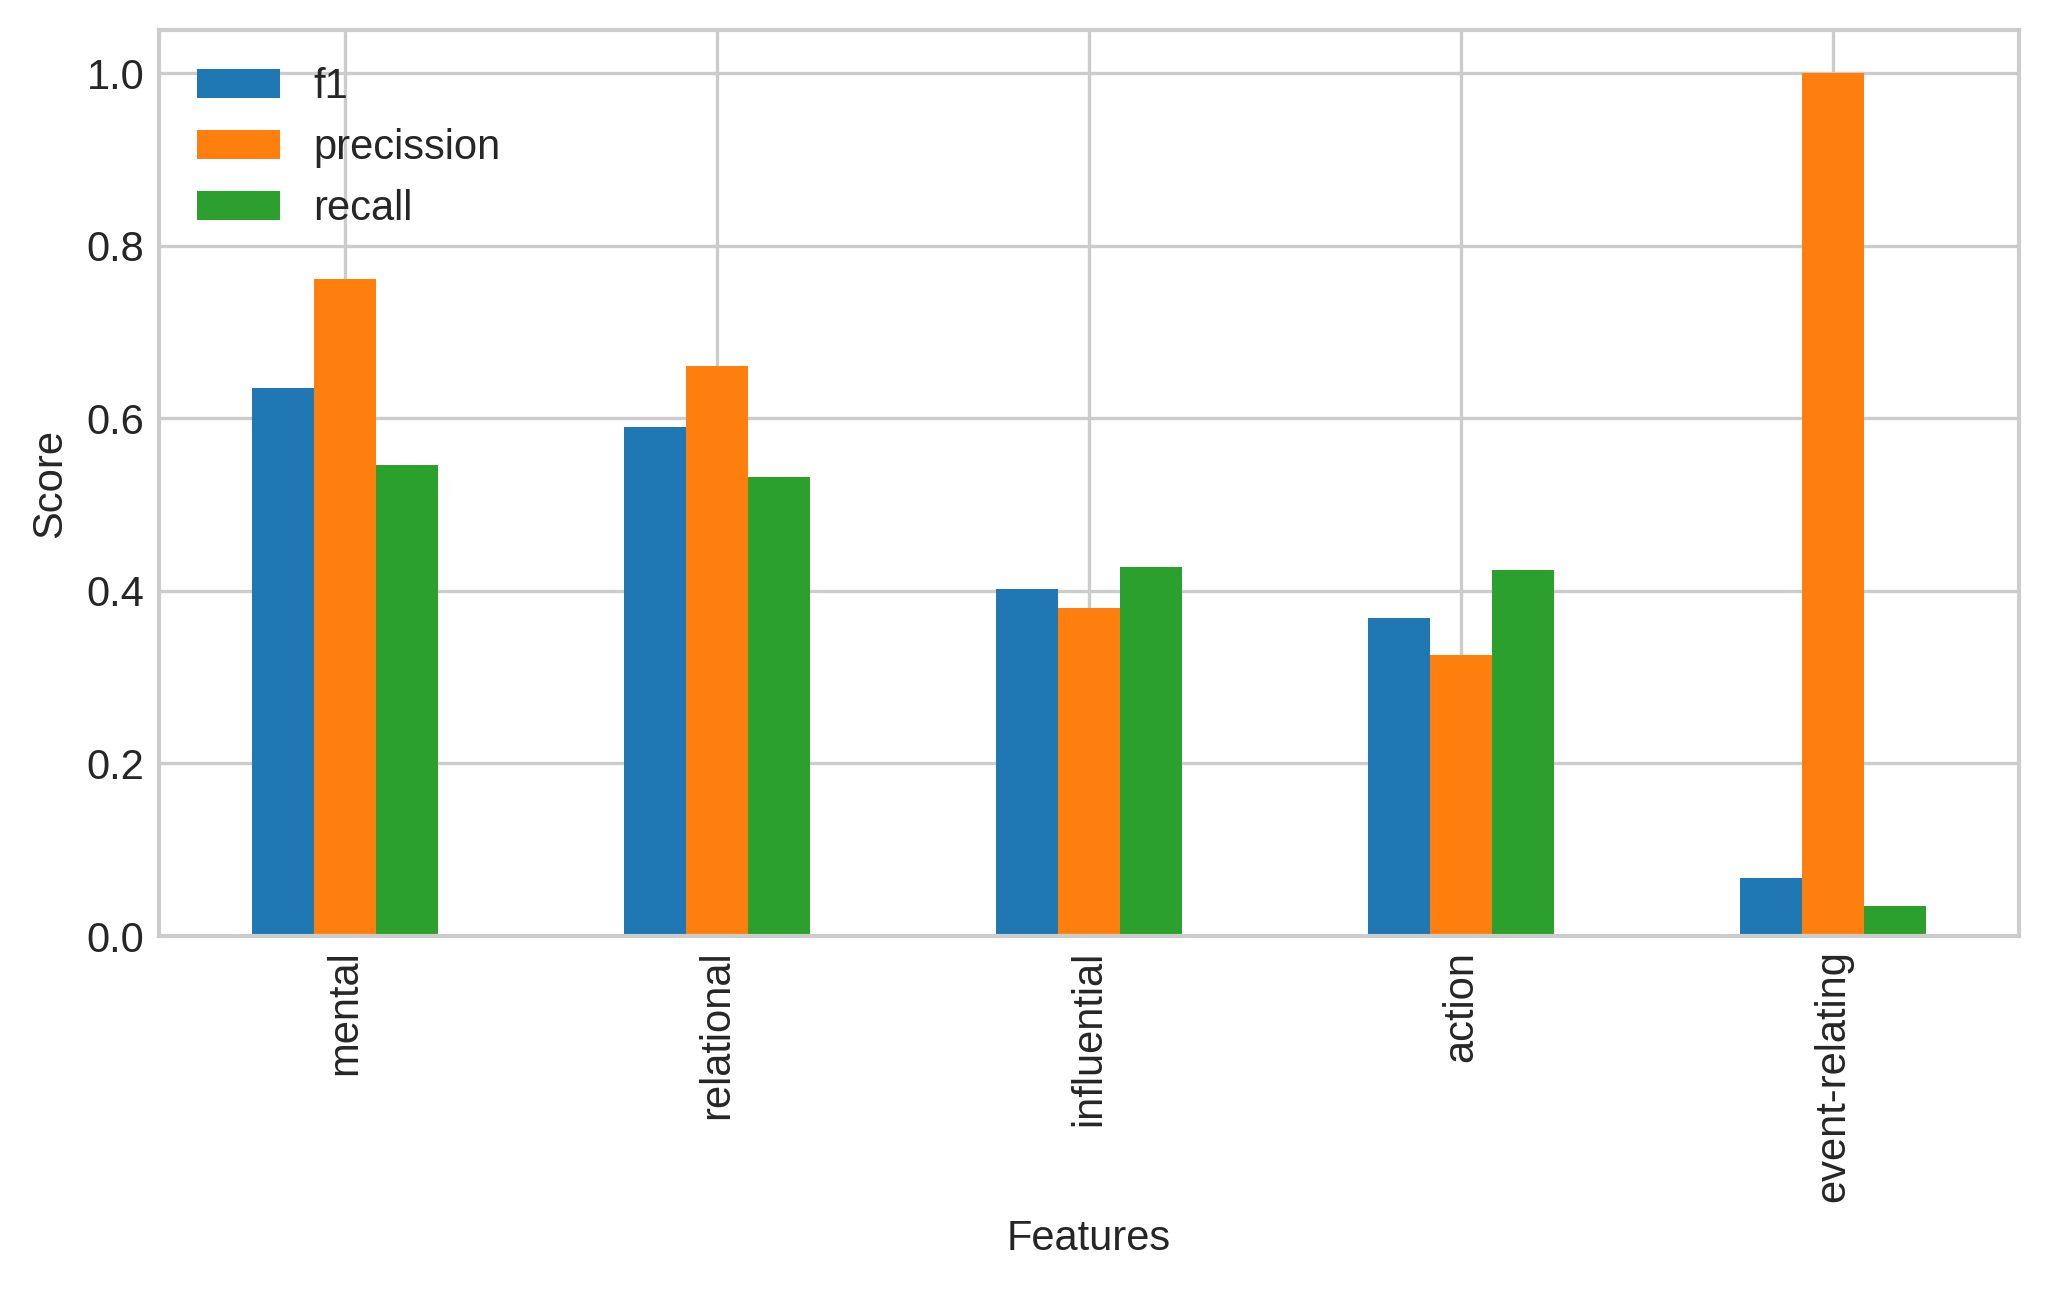
\includegraphics[width=.65\textwidth]{evaluation-results/figures/accuracy-semantic-process-type-f1}
    %    \caption{Bar chart of matched and non-matched (manual and parse) segments of the PROCESS-TYPE features}
        \caption{Bar chart of F1, precision and recall scores for PROCESS-TYPE features}
        \label{fig:process-types}
    \end{figure}
    
    \begin{figure}[!ht]
        \centering
        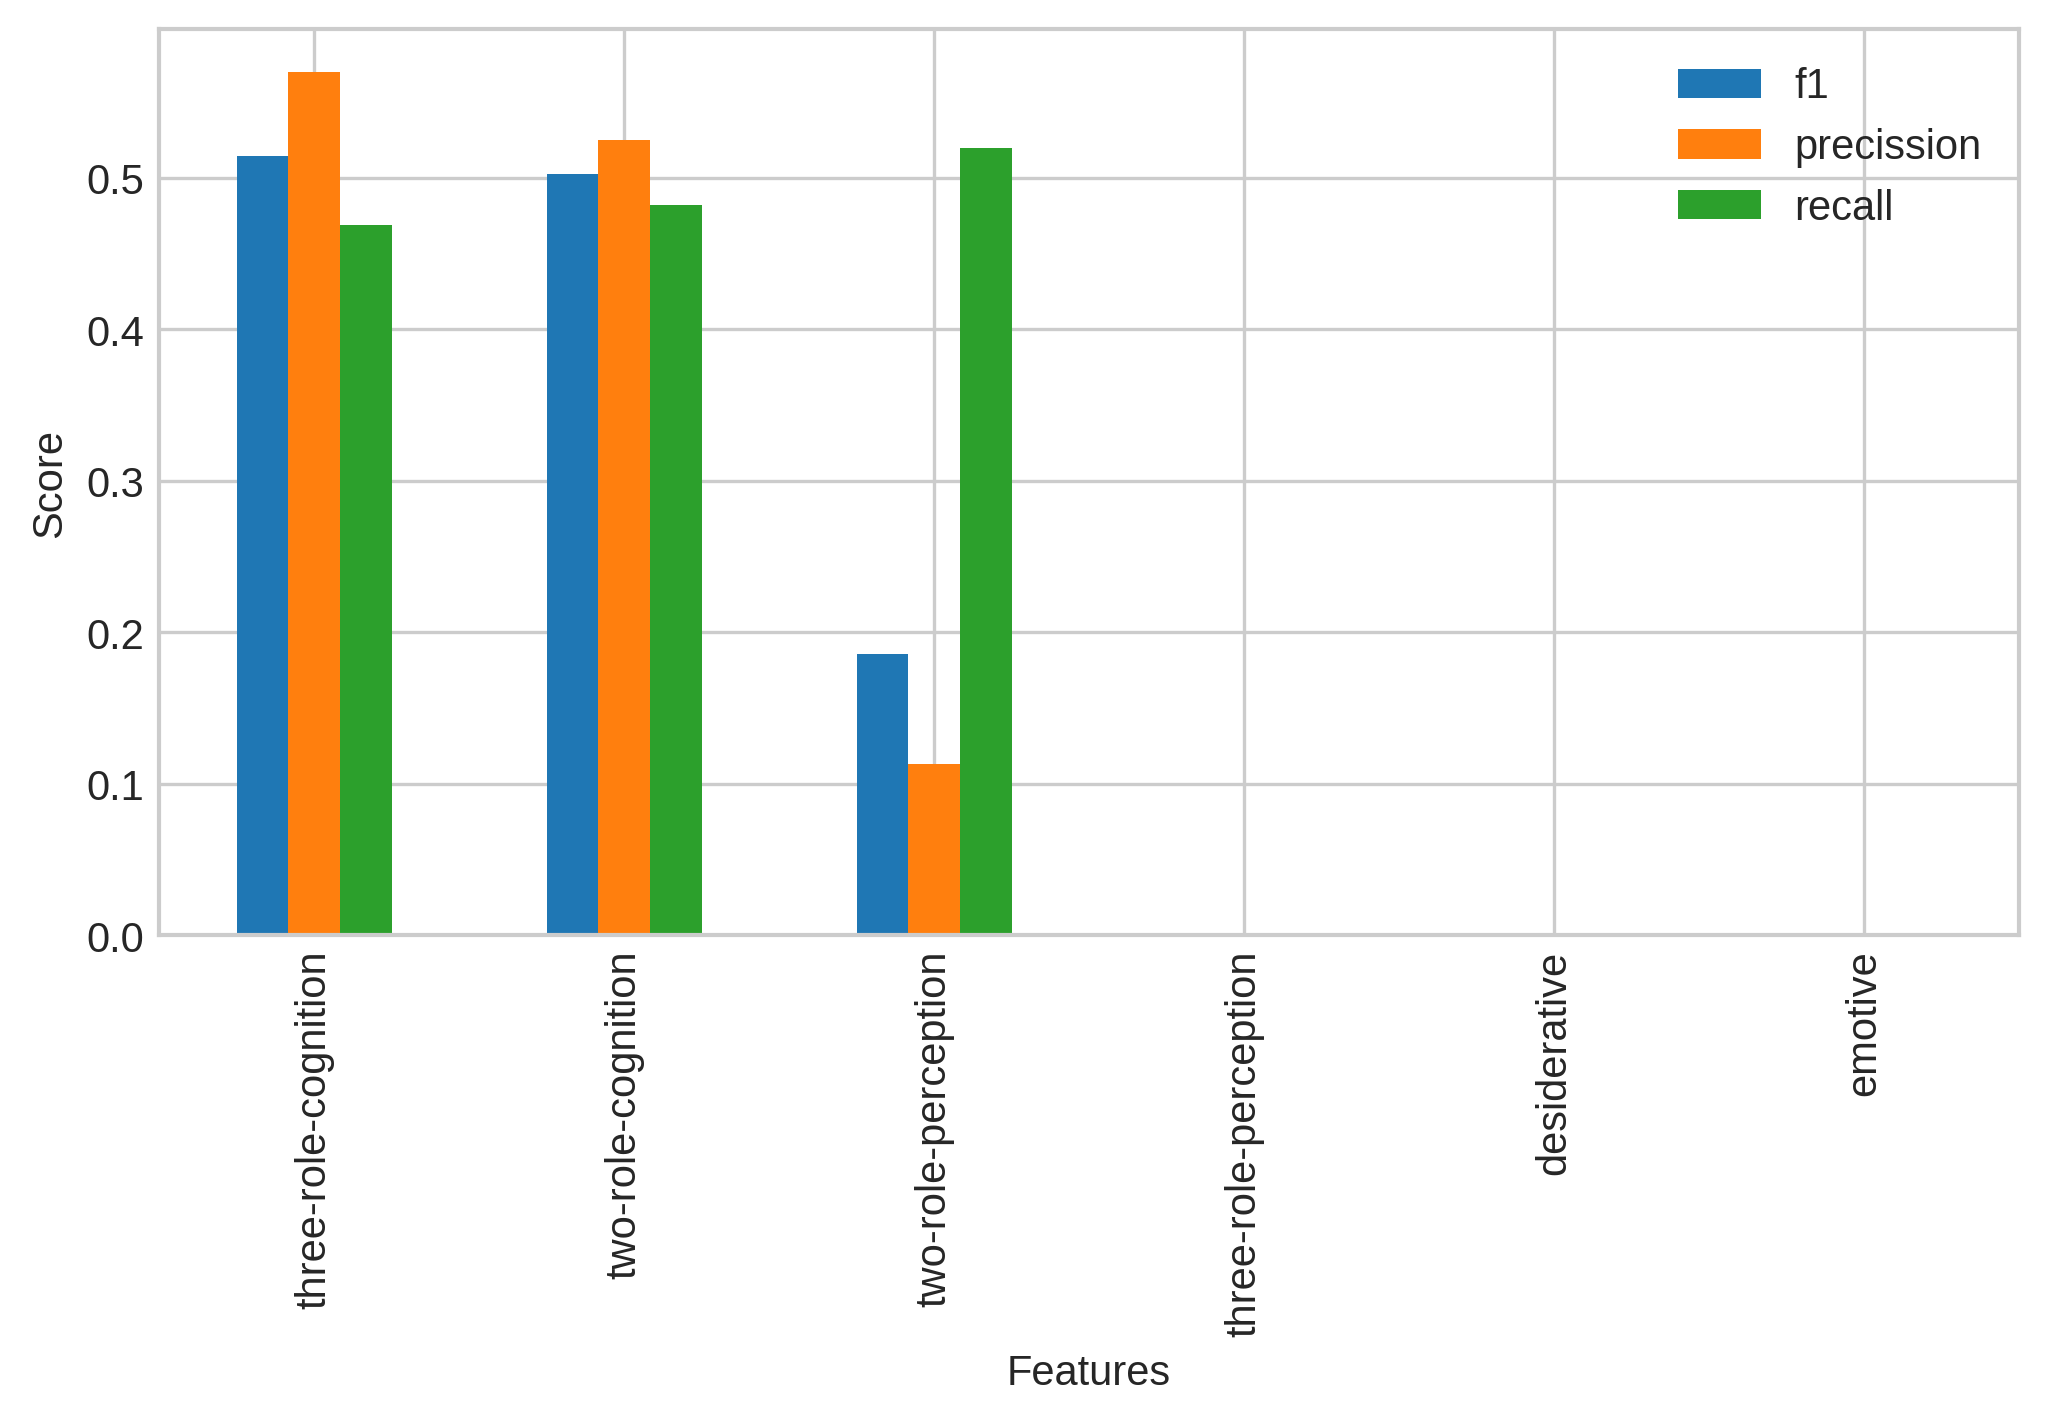
\includegraphics[width=.65\textwidth]{evaluation-results/figures/accuracy-semantic-mental-type-f1}
    %    \caption{Bar chart of matched and non-matched (manual and parse) segments of the MENTAL-TYPE features}
        \caption{Bar chart of F1, precision and recall scores for MENTAL-TYPE features}
        \label{fig:mental-types}
    \end{figure}
    
    \begin{figure}[!ht]
        \centering
        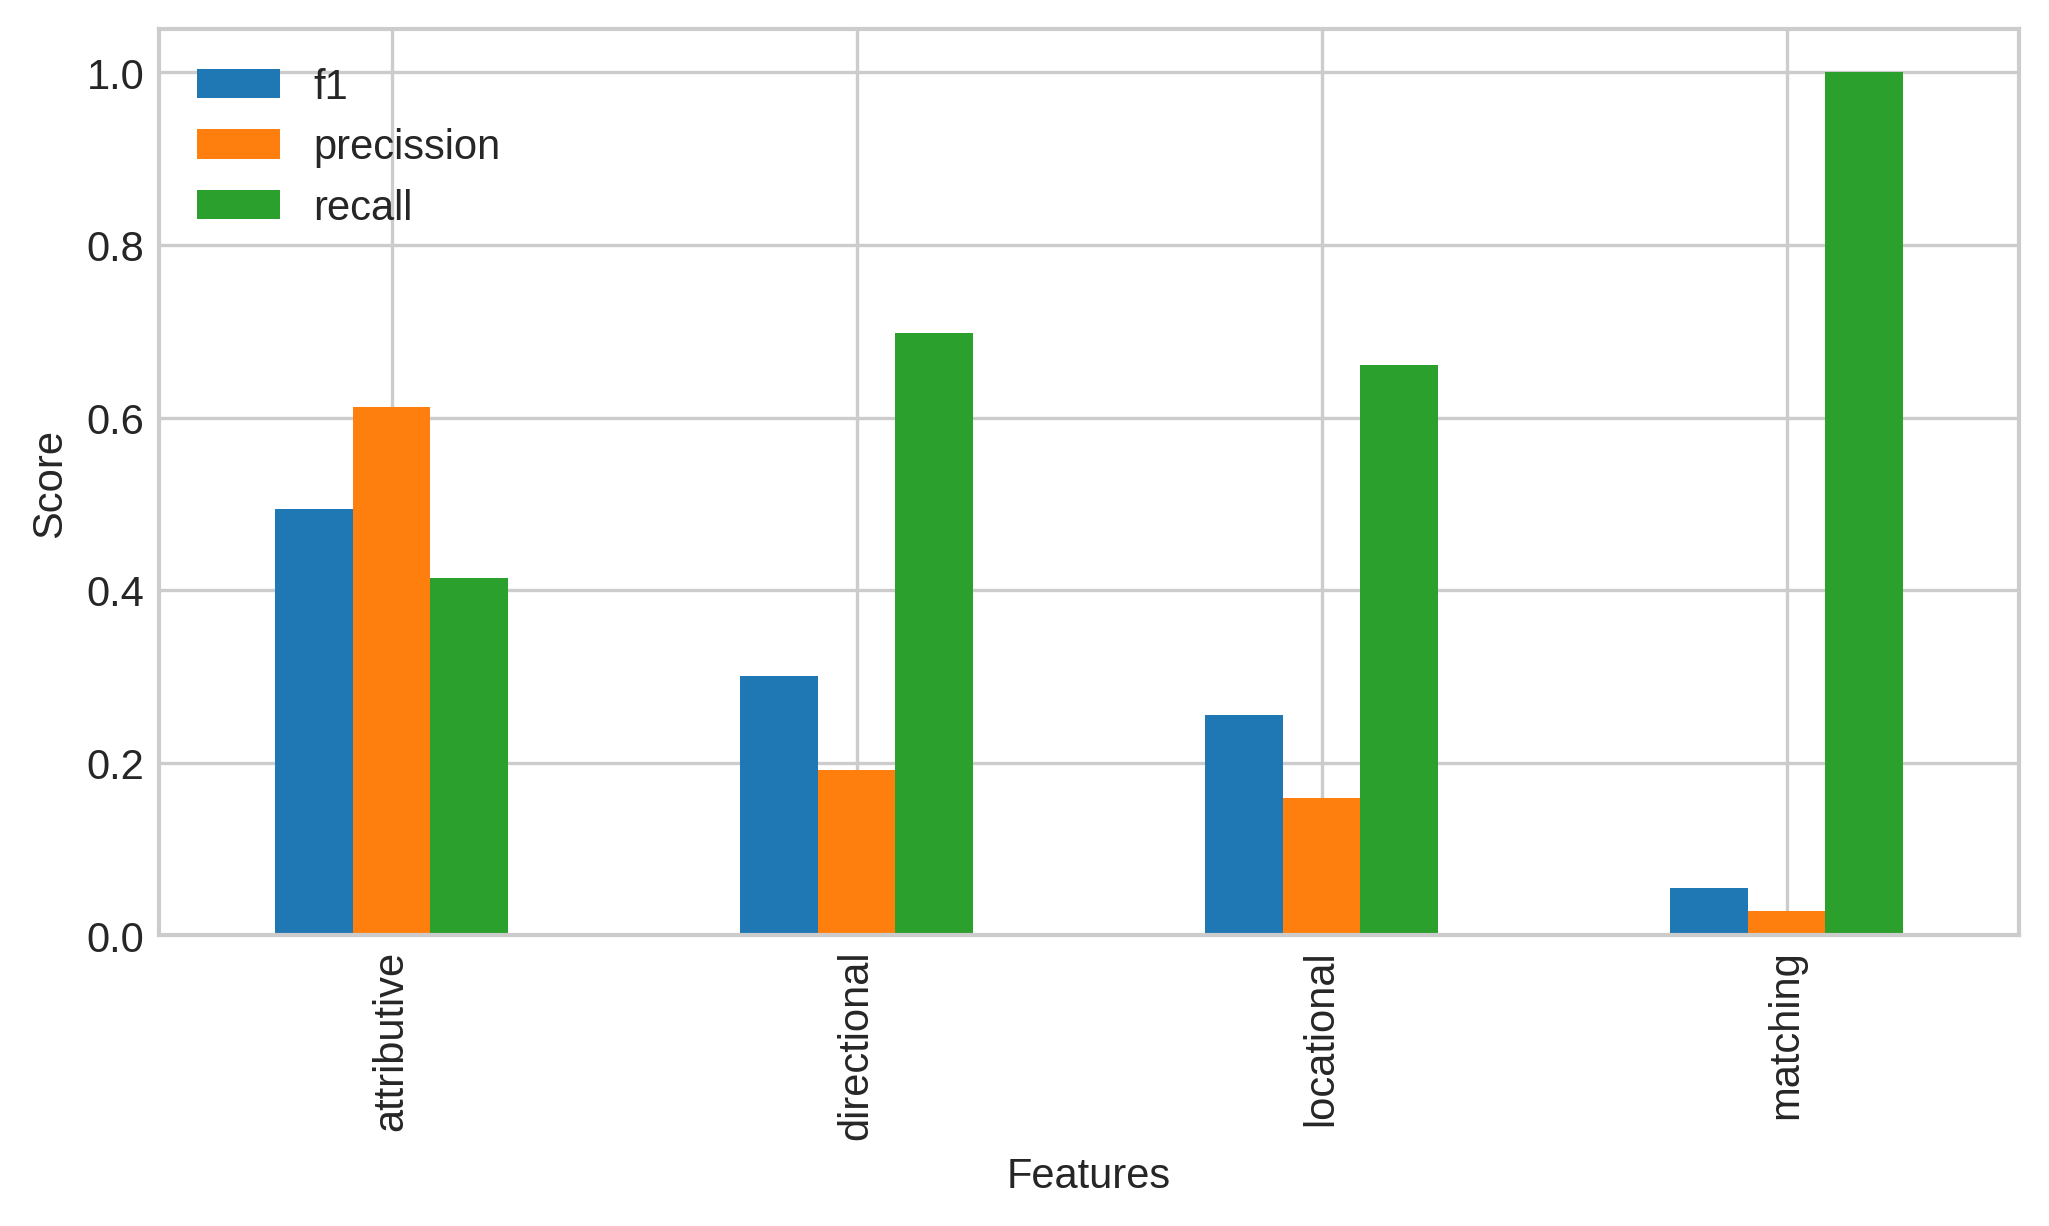
\includegraphics[width=.65\textwidth]{evaluation-results/figures/accuracy-semantic-relational-type-f1}
    %    \caption{Bar chart of matched and non-matched (manual and parse) segments of the RELATIONAL-TYPE features}
        \caption{Bar chart of F1, precision and recall scores for RELATIONAL-TYPE features}
        \label{fig:relational-types}
    \end{figure}

    \textit{Mental} and \textit{relational} processes are the ones with highest F_1 scores: 64\% and 59\%. They are followed by \textit{influential} and \textit{action} process types while results for the \textit{event-relating} are not conclusive because of the very small number of occurrences in the dataset. This can be seen in Figure \ref{fig:process-types} where the number of Matched segments (the left-most blue bar) is higher than the number of non matched Manual or Parse segments. This figure depicts the first part of the data in Table \ref{tab:features-transitivity}. The second and third parts are depicted in Figure \ref{fig:mental-types} and \ref{fig:relational-types}.

    Among the \textit{mental} processes, Figure \ref{fig:mental-types}, \textit{two} and \textit{three} role \textit{cognition} are parsed the best, whereas among \textit{relational} ones, Figure \ref{fig:relational-types}, the \textit{attributive} process type scores the highest while rest of them score quite low. This can be seen from the higher number of  non- matched segments for each process type depicted as orange and green bars in the middle and on the right (for every feature). 

    Table \ref{tab:ratios-mental} and \ref{tab:ratios-relational} provide each two pairs of ratios. They have very similar data content. Next I discuss the case of the mental process type only because the same applies to the case of relational processes and perhaps to other ones, but we lack data for testing this hypothesis. Thus, the first pair of ratios, provided in the lowest row, compares the number of segments with \textit{mental} feature to the number of segments with any sub-type of \textit{mental} feature (see Figure \ref{fig:mental-types}) (i.e. the aggregates over \textit{cognition}, \textit{perception}, \textit{emotive}, etc.). This ratio measures how well are the feature dependencies preserved across delicacy levels. The second pair of ratios, provided in the last column, compares the number of segments provided by the parser and to that available in corpus for both the mental feature and the sum of its sub-types. 

    Table \ref{tab:ratios-mental} shows that in the corpus the number of segments with \textit{mental} feature is almost one fourth higher than what the parser provides (72 \%). This result means that probably not all the instances of a mental process have been detected by the parser (i.e. 28\% undetected). The same comparison ran on the sub-types of \textit{mental} process shows diametrically opposite results, i.e. three fourths more parser generated results than in the corpus (172\%) which is an indication of false positives. A possible explanation is the correlation between increase in delicacy and uncertainty i.e. the more delicate features are less precise in the parser results. As mentioned in the beginning of the section, uncertainty this case is manifested as a disjunction set of equally possible options. Currently there is no ranking available based on degrees of confidence. Hence the parser provides multiple feature selections from the same system (in this case MENTAL-TYPE) for the same constituent whereas there should be a single one. In the future this needs to be addressed by introducing a discrimination mechanism for every system in the network. A possible approach is to integrate the frequencies available from the corpus.

   \begin{table}[!ht]
    \noindent
    \resizebox{0.98\linewidth}{!}{%
     \begin{minipage}[t]{0.495\textwidth}
         \centering
         \resizebox{0.995\textwidth}{!}{%  
             \begin{tabulary}{1.2\textwidth}{|C|c|c|c|}
                 \hline
                 \textbf{Features} & \textbf{Manual} & \textbf{Parse} & \textbf{/} \\ \hline
                 mental & 508 & 364 & \textbf{0.72} \\ \hline
                 mental sub-types (sum of) & 320 & 549 & \textbf{1.72} \\ \hline
                 \textbf{/} & \textbf{0.63} & \textbf{1.51} &  \\ \hline
             \end{tabulary}
         }
         \caption{The ratios between \textit{mental} segments and the sum of mental sub-type segments}
         \label{tab:ratios-mental}
     \end{minipage}%
     \quad
     \begin{minipage}[t]{0.495\textwidth}
         \centering
         %    \begin{table}[!ht]
         \resizebox{0.995\textwidth}{!}{%  
             \begin{tabulary}{1.2\textwidth}{|C|c|c|c|}
                 \hline
                 \textbf{Features} & \textbf{Manual} & \textbf{Parse} & \textit{\textbf{/}} \\ \hline
                 relational & 635 & 512 & \textbf{0.8} \\ \hline
                 relational sub-types (sum of) & 512 & 750 & \textbf{1.47} \\ \hline
                 \textit{\textbf{/}} & \textbf{0.8} & \textbf{1.47} &  \\ \hline
             \end{tabulary}
         }
         \caption{The ratios between \textit{relational} segments and the sum of mental sub-type segments}
         \label{tab:ratios-relational}
         %    \end{table}
     \end{minipage}
     }
    \end{table}

    If we look again at Table \ref{tab:ratios-mental} and compare the number of all mental sub-type occurrences (see Figure \ref{fig:mental-types}) to the number of mental type occurrences, then we see that the ratio is quite low (63\%). As the delicacy of the features increases fewer of these features are provided in the corpus. This is a direct manifestation of difficulty in annotating with ever more delicate features. This ratio, therefore, measures the degree of incompleteness at this level of delicacy. Comparing the same ratio for the parser generated segments we notice an opposite result (151\%). This is in fact another measurement of noise generated due to uncertainty when advancing to a more delicate features as explained above. 

    So far we have discussed the process types and now let's turn attention towards the features from the PARTICIPANT-ROLE-TYPE system. Table \ref{tab:features-participant-role} presents the evaluation data and Figure \ref{fig:participant-roles-f1} depicts the precision, recall and F_1 score for each role sorted according to F_1 score in descending order while Figure \ref{fig:participant-roles} depicts the absolute number of segments for each feature.

    \begin{table}[!ht]
        \resizebox{0.95\textwidth}{!}{%  
        \begin{tabular}{|c|c|c|c|c|c|c|c|c|c|}
            \hline
            \textbf{Feature} & \textbf{Match} & \textbf{\begin{tabular}[c]{@{}c@{}}Manual\\ nm\end{tabular}} & \textbf{\begin{tabular}[c]{@{}c@{}}Parse\\ nm\end{tabular}} & \textbf{Precision} & \textbf{Recall} & \textbf{F1} & \textbf{\begin{tabular}[c]{@{}c@{}}\%Total \\ matched\end{tabular}} & \textbf{\begin{tabular}[c]{@{}c@{}}\%Manual\\ nm\end{tabular}} & \textbf{\begin{tabular}[c]{@{}c@{}}\%Parse\\ nm\end{tabular}} \\ \hline
            emoter & 91 & 70 & 57 & 0.61 & 0.57 & 0.59 & 5.48 & 43.48 & 38.51 \\ \hline
            phenomenon & 359 & 223 & 294 & 0.55 & 0.62 & 0.58 & 21.60 & 38.32 & 45.02 \\ \hline
            carrier & 267 & 263 & 244 & 0.52 & 0.50 & 0.51 & 16.06 & 49.62 & 47.75 \\ \hline
            possessive & 75 & 48 & 99 & 0.43 & 0.61 & 0.51 & 4.51 & 39.02 & 56.90 \\ \hline
            cognizant & 82 & 84 & 104 & 0.44 & 0.49 & 0.47 & 4.93 & 50.60 & 55.91 \\ \hline
            agent & 267 & 210 & 428 & 0.38 & 0.56 & 0.46 & 16.06 & 44.03 & 61.58 \\ \hline
            possessed & 71 & 24 & 155 & 0.31 & 0.75 & 0.44 & 4.27 & 25.26 & 68.58 \\ \hline
            attribute & 162 & 241 & 170 & 0.49 & 0.40 & 0.44 & 9.75 & 59.80 & 51.20 \\ \hline
            destination & 18 & 10 & 121 & 0.13 & 0.64 & 0.22 & 1.08 & 35.71 & 87.05 \\ \hline
            affected & 93 & 70 & 663 & 0.12 & 0.57 & 0.20 & 5.60 & 42.94 & 87.70 \\ \hline
            location & 17 & 40 & 226 & 0.07 & 0.30 & 0.11 & 1.02 & 70.18 & 93.00 \\ \hline
            source & 1 & 6 & 13 & 0.07 & 0.14 & 0.10 & 0.06 & 85.71 & 92.86 \\ \hline
            created-phenomenon & 29 & 12 & 647 & 0.04 & 0.71 & 0.08 & 1.74 & 29.27 & 95.71 \\ \hline
            path & 1 & 4 & 19 & 0.05 & 0.20 & 0.08 & 0.06 & 80.00 & 95.00 \\ \hline
            range & 11 & 19 & 240 & 0.04 & 0.37 & 0.08 & 0.66 & 63.33 & 95.62 \\ \hline
            affected-carrier & 33 & 28 & 899 & 0.04 & 0.54 & 0.07 & 1.99 & 45.90 & 96.46 \\ \hline
            affected-possessed & 20 & 6 & 575 & 0.03 & 0.77 & 0.06 & 1.20 & 23.08 & 96.64 \\ \hline
            affected-cognizant & 22 & 34 & 624 & 0.03 & 0.39 & 0.06 & 1.32 & 60.71 & 96.59 \\ \hline
            manner & 1 & 7 & 25 & 0.04 & 0.12 & 0.06 & 0.06 & 87.50 & 96.15 \\ \hline
            perceiver & 10 & 8 & 344 & 0.03 & 0.56 & 0.05 & 0.60 & 44.44 & 97.18 \\ \hline
            agent-carrier & 17 & 12 & 745 & 0.02 & 0.59 & 0.04 & 1.02 & 41.38 & 97.77 \\ \hline
            created & 3 & 15 & 228 & 0.01 & 0.17 & 0.02 & 0.18 & 83.33 & 98.70 \\ \hline
            matchee & 1 & 2 & 91 & 0.01 & 0.33 & 0.02 & 0.06 & 66.67 & 98.91 \\ \hline
            agent-perceiver & 6 & 1 & 657 & 0.01 & 0.86 & 0.02 & 0.36 & 14.29 & 99.10 \\ \hline
            agent-cognizant & 2 & 3 & 633 & 0.00 & 0.40 & 0.01 & 0.12 & 60.00 & 99.69 \\ \hline
            affected-perceiver & 1 & 0 & 544 & 0.00 & 1.00 & 0.00 & 0.06 & 0.00 & 99.82 \\ \hline
            affected-destination & 1 & 0 & 593 & 0.00 & 1.00 & 0.00 & 0.06 & 0.00 & 99.83 \\ \hline
            affected-emoter & 1 & 0 & 631 & 0.00 & 1.00 & 0.00 & 0.06 & 0.00 & 99.84 \\ \hline
            affected-path & 0 & 0 & 494 & 0.00 &  &  & 0.00 &  & 100.00 \\ \hline
            affected-source & 0 & 0 & 490 & 0.00 &  &  & 0.00 &  & 100.00 \\ \hline
        \end{tabular}
    }
    \caption{The evaluation statistics available for the PARTICIPANT-ROLE-TYPE system from the TRANSITIVITY system network}
    \label{tab:features-participant-role}
    \end{table}

    \begin{figure}[!ht]
        \centering
        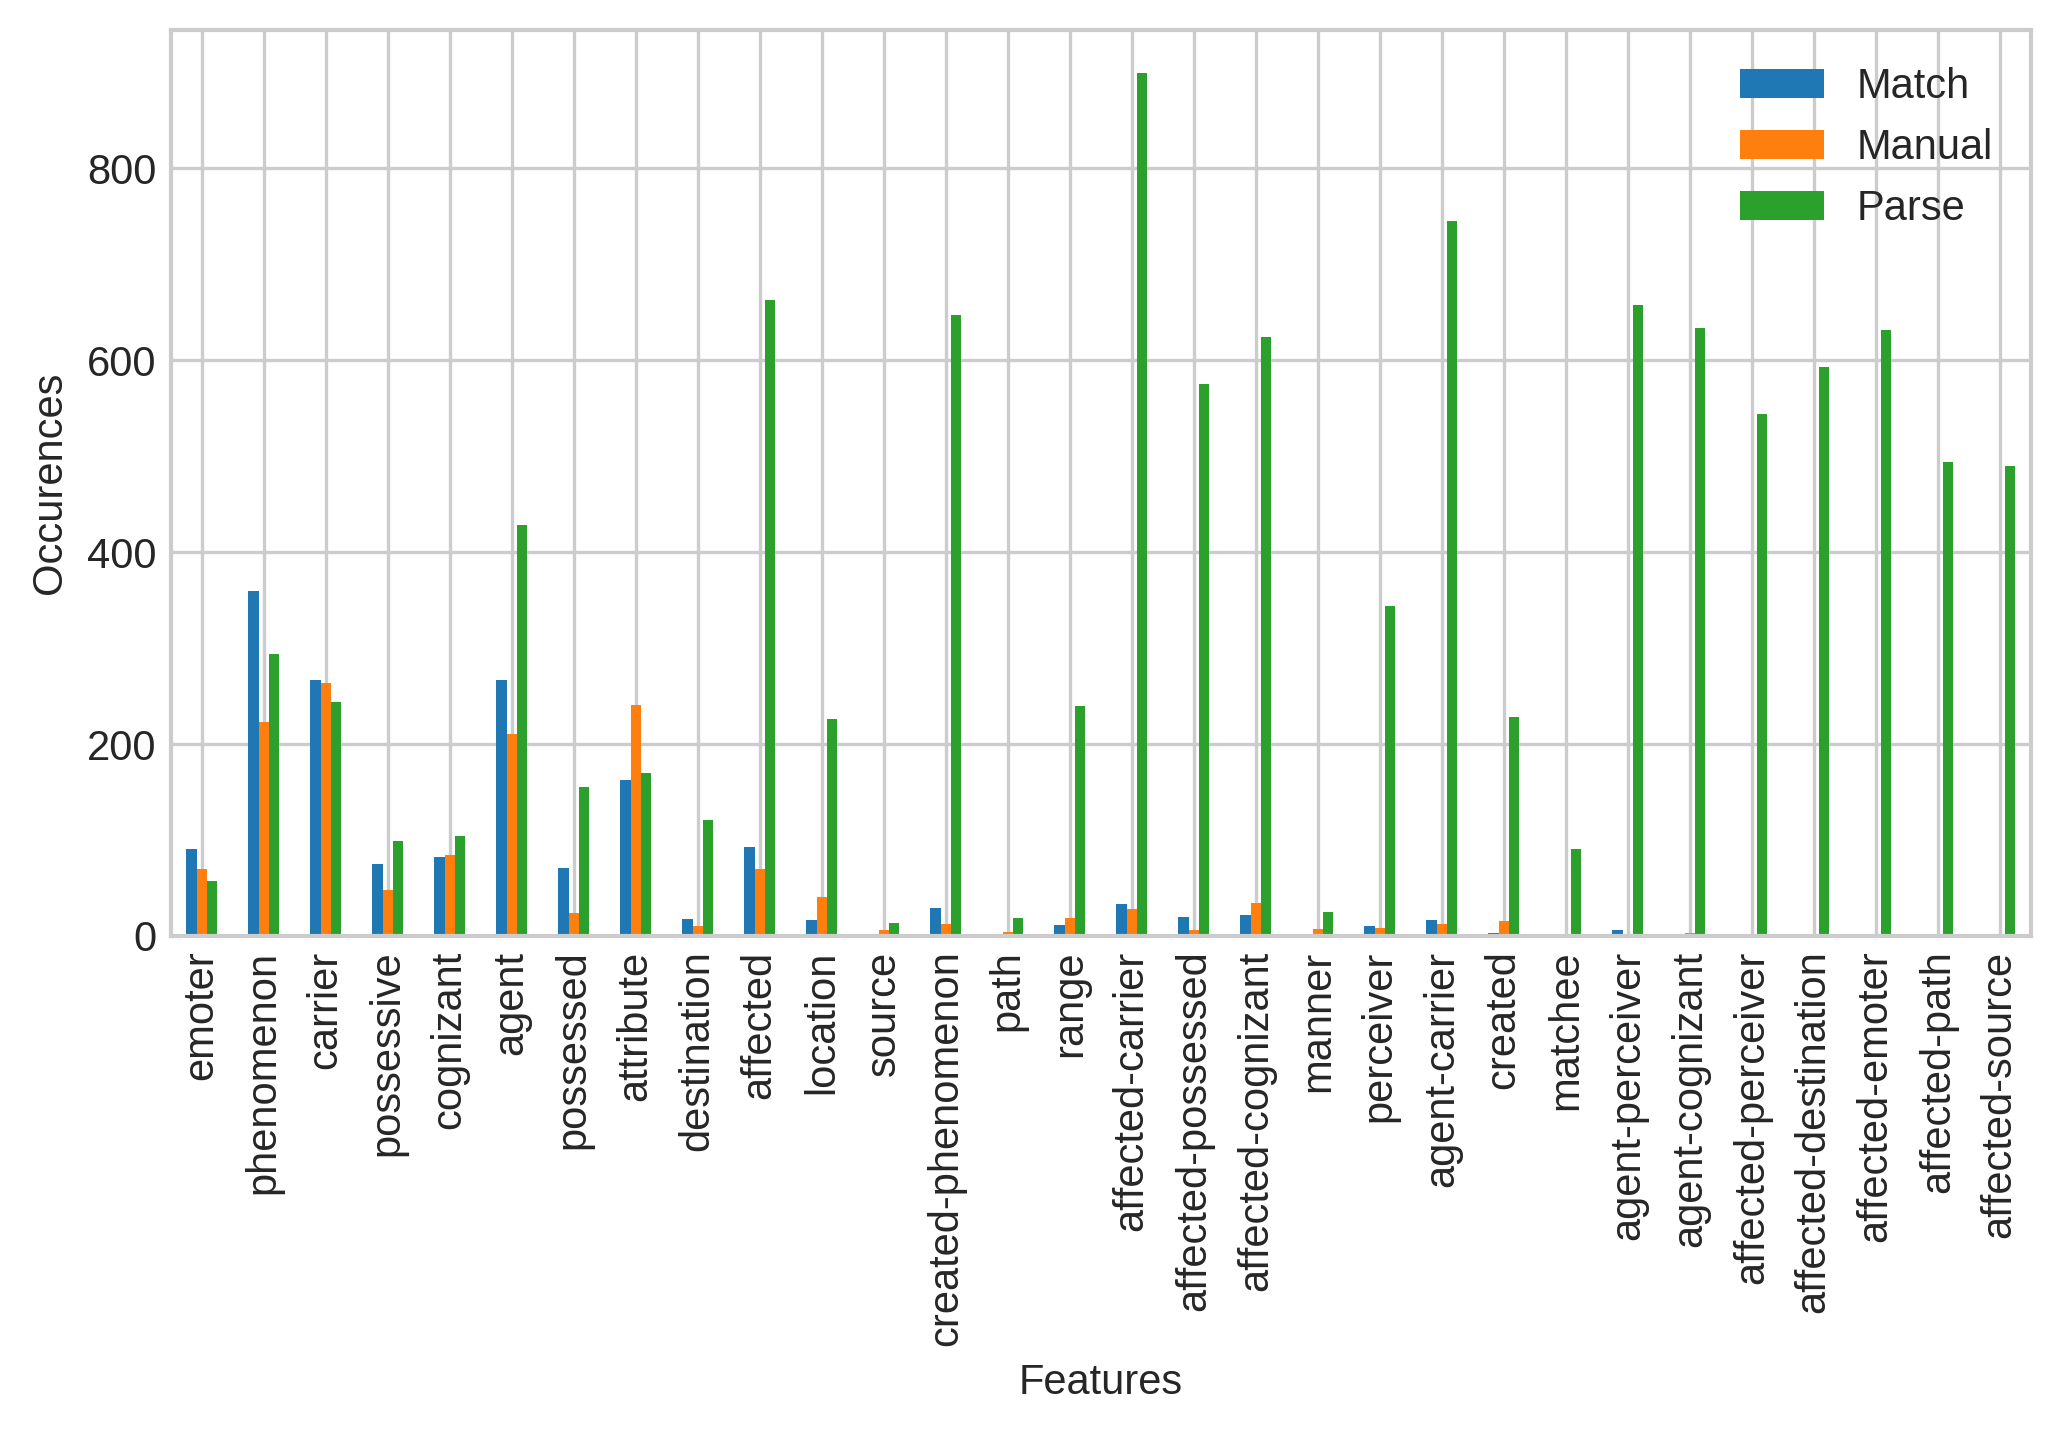
\includegraphics[width=.995\textwidth]{evaluation-results/figures/accuracy-semantic-participant-type1}
        \caption{Bar chart of matched and non-matched (manual and parse) segments of the PARTICIPANT-TYPE features}
        \label{fig:participant-roles}
    \end{figure}
    \begin{figure}[!ht]
        \centering
        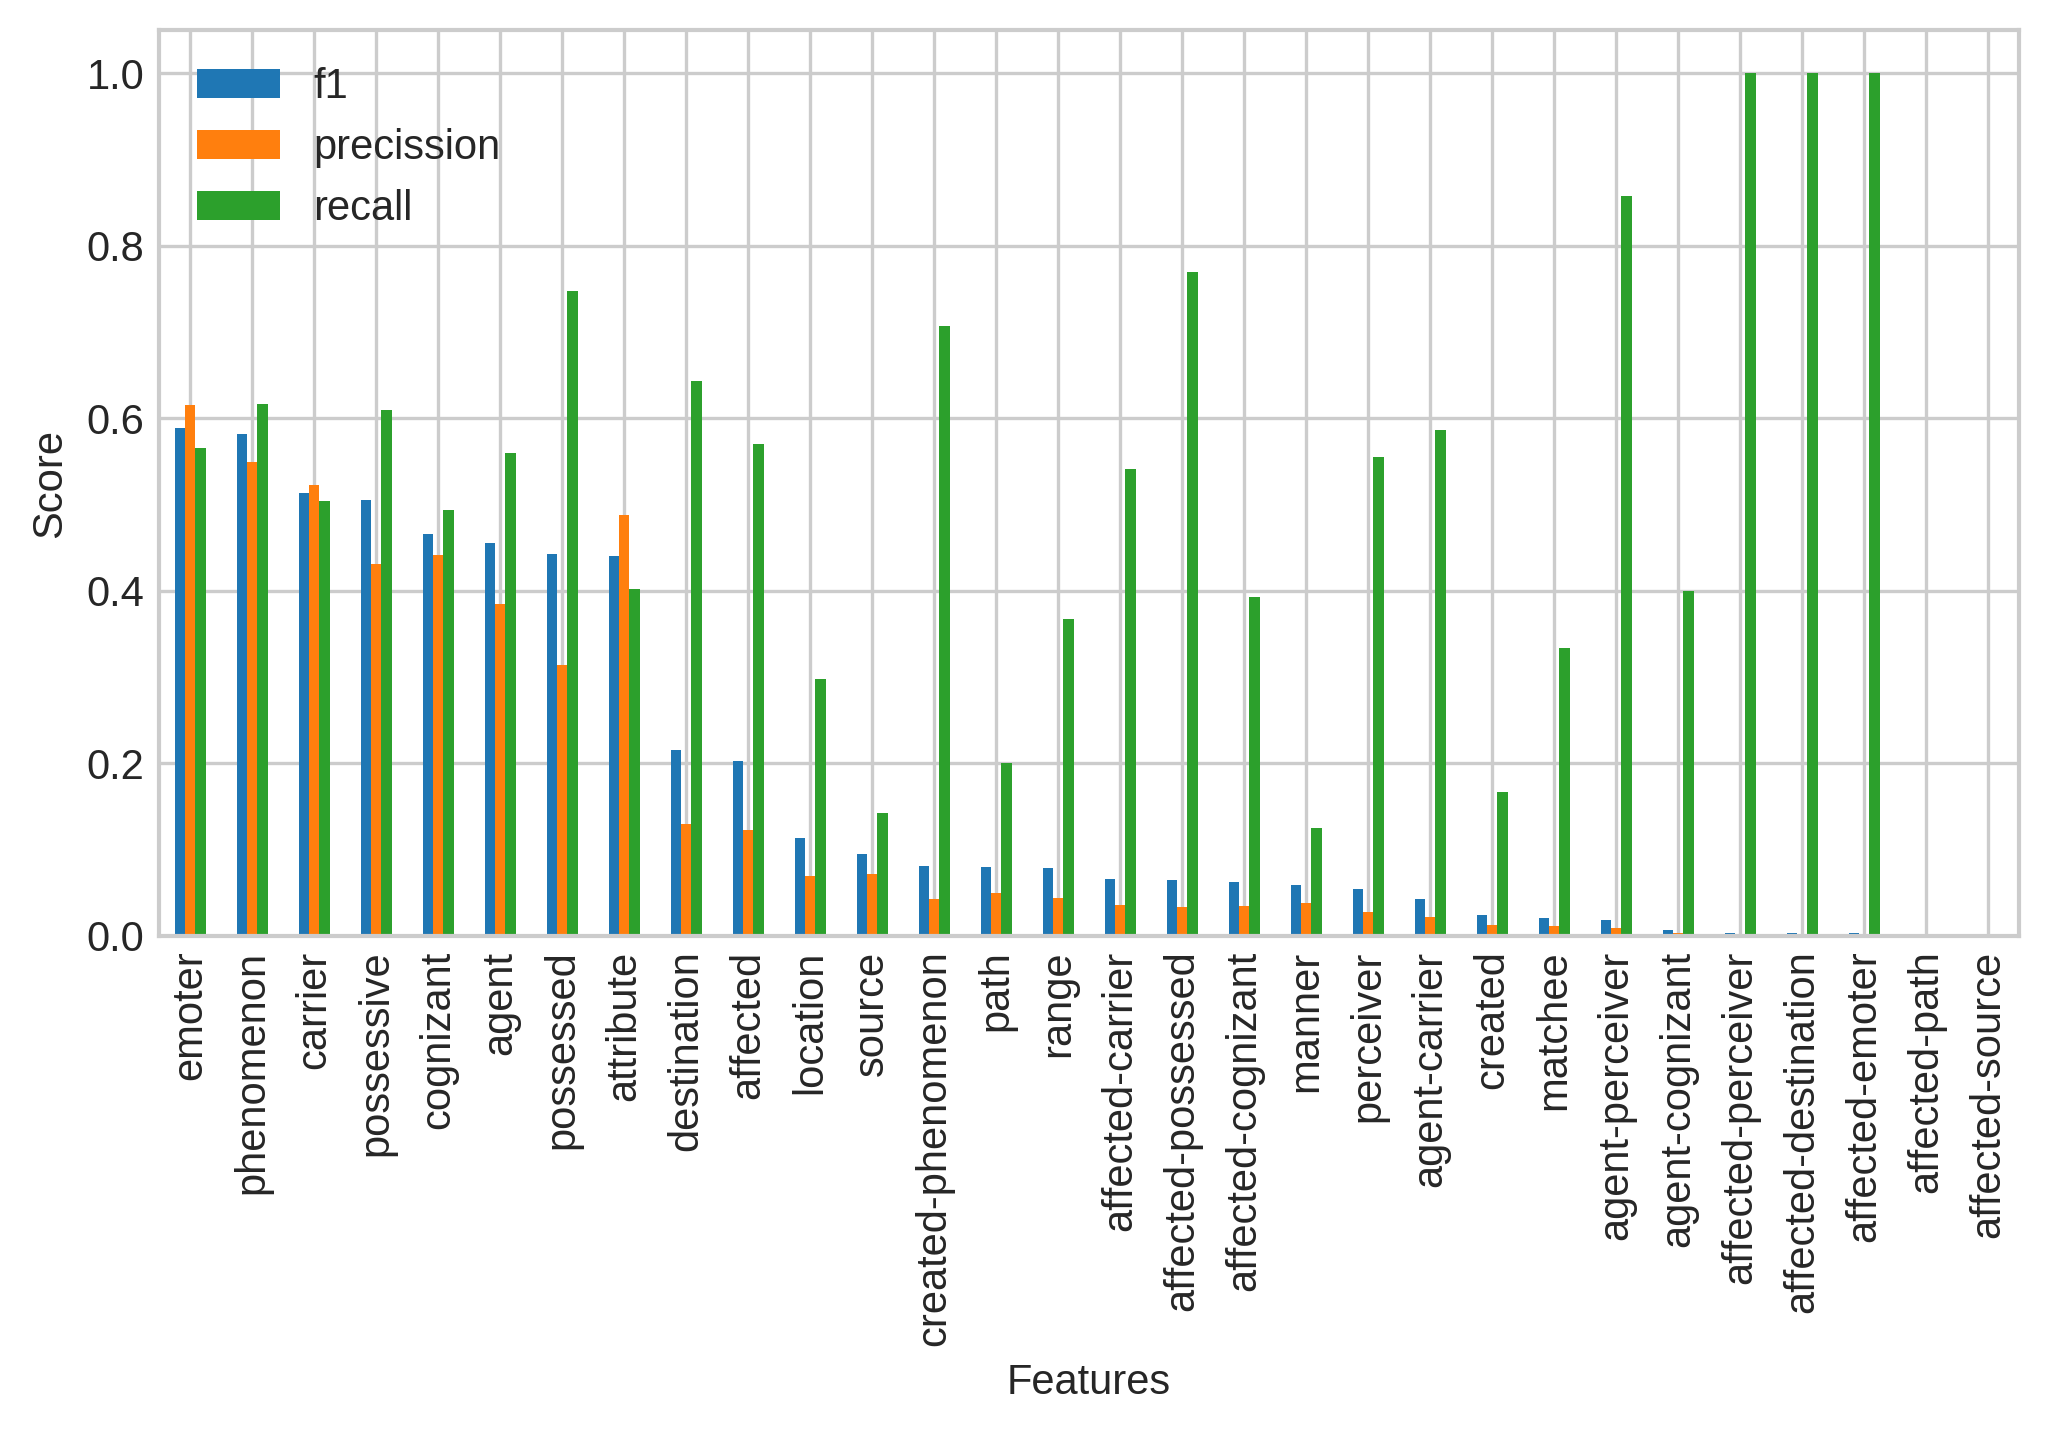
\includegraphics[width=.995\textwidth]{evaluation-results/figures/accuracy-semantic-participant-type1-f1}
        \caption{Bar chart of F1, precision and recall scores for the PARTICIPANT-TYPE features}
        \label{fig:participant-roles-f1}
    \end{figure}

    A suite of eight features: emoter, phenomenon, carrier, possessive, cognizant, agent, possessed and attribute have F_1 scores descending from almost 60\% to 44\%. Destination and affected features follow with half of the previous (20\%) and then the score halves again to 11\% continuing to descend towards zero. As the F_1 score decreases we can notice that some features display high recall spikes. This is a manifestation of the assignment of multiple roles to the same participant for the reasons explained above for the process types. 

    From the data presented in Figure \ref{fig:participant-roles-f1} we can conclude that only one third of the participant roles can be considered usable with a reasonable level of confidence. Yet in Figure \ref{fig:participant-roles} we can see that there is also a serious lack of data, which can explain a part of the low F_1 scores. A hypothesis that I put forward here is that in a larger corpus, with broader coverage over the participant roles, the scores for the rare features would considerably improve. Nonetheless an investigation is needed for Transitivity graph patterns generated from the PTDB, especially on the features exhibiting recall spikes. The next section concludes this evaluation chapter.

\section{Discussion}
\label{sec:evaluation-discussion}
    In this chapter we have discussed how the empirical evaluation of Parsimonious Vole parser has been conducted. The stage is set through a general presentation of the corpora and what the task at hand is, i.e. identifying and comparing segments available in the manually annotated corpus to those generated automatically by the parser. 

    The first issue is deciding when two segments are the same. This is addressed in Section \ref{sec:segment-alignment} to \ref{sec:stable-marriage} covering a method to convert parser constituents into segments, reading the corpus segments and an algorithm, derived from the stable marriage problem, for matching segments  to detect the amount of overlap.

    The results are presented and analysed in Section \ref{sec:results}. This starts with general findings where we can see that 83\% of the segment have identical spans or are slightly shifted. The analysis advances to determine which elements are shifted and sets the foundation for future developments and corrections in the software. Next a syntactic and semantic analysis of constituent elements and systemic features are presented. 

    The syntactic constituents score between 50\% and 90\% F_1 measure whereas the semantic ones are more stable scoring between 79\% and 82\% F_1 measure. These results can be seen in Section \ref{sec:syntactic-constituents} and \ref{sec:semantic-constituents}. When it comes to systemic features evaluation the results vary a lot not only between features at different levels of delicacy but also between sibling features within the same system. Analysis is provided in Section \ref{sec:syntactic-features} and \ref{sec:semantic-features}.

    Further investigation needs to be conducted to determine the sources and types of errors, shortcomings and potential approaches to improve both the corpus and parser. 

    Because each of the current corpora has a single main annotator, a valuable future task is to add multiple annotators and establish agreement between them. Also, the corpora size is very small and many systemic features are missing or under-represented. For example event relating, environmental and other processes are missing from the corpus just like the distinctions of action types. It would be interesting to extend the annotation and include more MOOD features to study how they vary and how accurately the parser detects them. 

    Each corpus has been created by a single author providing both syntactic and semantic annotations. This fact is an indication that the current corpus does not constitute a reliable golden standard and a more grounded corpus needs to be developed in the future with multiple independent authors and high inter-annotator agreement. Therefore, the results should be considered indicative and by no means representative of the parser performance or corpus quality. Nevertheless, this is already a good starting point for investigations of certain grammar areas with considerable low performance in order identify and resolve potential problems. Also, this evaluation is the first one and constitutes the baseline for further incremental developments.